\chapter{Growth and development of the socio-economic space}
\label{ch:relationaltheory}

Chapter~\ref{ch:relationalperspective} developed the fundamental definitions, axioms, and hypotheses required for a theoretical discussion of social and economic interaction within the relational perspective. This perspective hinges on the attributes of the economic agent---and thus the social actor---where we assume the endowment of both preferences and production abilities with learning effects within all individuals. The interaction between consumer-producers propagates the emergence of a social division of labour. This division of labour is founded on increasing returns to specialisation, gains from trade, the presence of socio-economic roles that are derived from the existence of a governance system, and trust in the elements of the governance system itself that solidify ones embeddedness and allows for functional economic interactions.

This chapter builds directly on the initial discussions of the relational perspective. In doing so we introduce the notion of a \emph{socio-economic space} within which all elements of the relational perspective are contained and all economic interactions occur. We note how a socio-economic space can \emph{grow} through changes in population and technological parameters, and \emph{develop} through major alterations of institutional elements of the governance system. These changes are also reflected in the networked interaction infrastructure of the socio-economic space and the overall utility derived from exchange within society as a whole.

An important element for the development of a socio-economic space is the role of the \emph{entrepreneur} and the process of \emph{entrepreneurship}. These concepts are initially discussed within this chapter and subsequently discussed in more detail in Chapter~\ref{ch:entrepreneurship} of the monograph. Entrepreneurship, we claim, is important for discussions on economic development and is linked directly to insights on positional power, the formation of new socio-economic roles, and the deepening of the division of labour.

\paragraph{Chapter outline.}

The purpose of this chapter is to provide a formal and conceptual discussion on the socio-economic space using insights discussed previously. We also illustrate the growth and development, and thus an effect of entrepreneurship and the entrepreneurial function, within the socio-economic space through the use of computational simulations. This chapter is therefore partitioned into four sections. The first provides a discussion of the socio-economic space which acts as an environment where economic agents interact and subsequently construct interaction infrastructures. Section two discusses theoretical and representative states of the socio-economic space. Section three considers the growth and development of the socio-economic space; in particular we discuss the notions of entrepreneurship and entrepreneurial function within the relational perspective. Finally, we provide simulations of the growth and development of the socio-economic space.

\section{The socio-economic space} \label{sec:socio-economicspace}

All economic relationships and interactions are socially embedded and occur within some well-defined space. This interaction space is termed as a socio-economic space, which refers to \emph{a set of economic agents engaged in a collection of general economic interactions and hierarchical relations that operate with respect to some well-defined governance system}. As such the socio-economic space contains economic agents, interaction infrastructures, and a governance system guiding the formation of these relationships. The importance of a governance system to guide social and economic interactions fits with the notion of an \emph{imagined community}, a concept that highlights the importance of a socially accepted and trusted governance system in harmonising interactions.

\subsection{A socio-economic space as an imagined community}

Within contemporary society we consider economies and socio-economic spaces as analogous to geographical, political, or legal entities; such as countries, nations, regions, cities, or firms. Within a more primitive economies we may consider these spaces as tribes and families.

In the most general terms a socio-economic space is an `imagined community'; a concept coined by Benedict \citet[p.~6--7]{Anderson1983b} who hypothesised that a nation is a, ``community socially constructed, imagined by the people who perceive themselves as part of that group''. Political and legal representation occurs and may solidify people's mental state however, at its core, a nation or country is a fictional and thus imagined entity. An imagined community is different from an actual community because it is not---and, for practical reasons, cannot be---based on everyday interaction between its members. It is based on notional trust and a socially accepted governance system, which becomes increasingly important as the space develops and becomes and more complex.

Members hold in their minds a mental image of their affinity. As Anderson puts it, a nation is imagined due to the fact that individuals that make up the community will never know or even see most other individuals, but in the minds of each lives the image of their community. There is some form of communal consciousness. Members of the community will, most likely, never know each of the other members face-to-face. However, they may have similar interests or identify as part of the same nation: they may be recognised by the same elements of the governance system, such as embedded and recognised socio-economic roles, behavioural rules, religion, cultural norms, and language, all of which facilitates primitive interaction. Furthermore, `media' reinforces imagined communities.

Anderson's main idea is that nations are fundamentally defined by a socially accepted and embedded mind set: by elements of the governance system that are adopted by members of the community. Importantly, we hypothesise that a socio-economic space is nothing more than a networked community that conform to similar elements of governance. It is also apparent that there must be strong institutional trust within the society when conducting socio-economic interactions and, as the imagined community expands in terms of population and functional economic relationships, there is specifically an increased requirement for strong levels of notional trust. Thus as an imagined community expands, not only does the governance system and the elements it comprises need to become more structured, formal, and hierarchical; but as it expands social trust in the elements become increasingly more important for cohesive long-term social and economic interactions. 

A functional socio-economic space, characterised by high levels of notional trust and a well-defined and socially understood governance system reduces interaction inefficiencies and facilitates interaction. Specifically, following from notions discussed previously\footnote{See subsection \ref{interactionGovernanceSystem}. } we see that a socio-economic space consisting of a well-defined governance system facilitates wealth-generation and the coordination of the division of labour to perform a specific output.

\subsection{Representing the socio-economic space}

A socio-economic space represents the essence of a socially structured economy. When discussing socially structured economies and markets Mark \citet{Granovetter1985, Granovetter2005} and John \citet{Lie1997} criticised the under-socialisation of traditional neoclassical economics and the apparent over-socialisation of new institutional economics. They claimed that, whereas neoclassical economics is shorn of all social interaction and socially constructed institutions, NIE gives too much emphasis to the command of institutional forces over the actions and organisation of agents and societies. They suggest, along with other works in the economic sociology literature \citep{DiMaggio1988, Swedberg2000, Battilana2006}, that agents have an ability, either collectively or individually, to manipulate elements of the institutional framework. This is, in their perspective, how society develops and, importantly, this `development' does not have to be for the benefit of society as a whole.

We maintain this perspective of a two-way interaction between institutions and agents, and suggest that economic agents have the ability to alter elements of the governance system, and therefore the mechanisms in which to do and enforce trade and the allocation of wealth throughout society. This alteration of the elements of the governance system is the essence of \emph{entrepreneurship}.

\subsubsection{Schematic representation of the socio-economic space} \label{subsubsec:schematicRepresentation}

The socio-economic space represents a population of economic agents, who each assume a socio-economic role, embedded in a governance system of institutions that guides the behaviours and actions of these economic agents. This behaviour leads to an interaction infrastructure that consists of a variety of economic interactions and trade relationships.

Importantly there exists a two-way relationship between the economic agents in the population and the set of institutions in the governance system. The relationship can be represented graphically by the schematic in Figure~\ref{spacestructure}, which is clearly reminiscent of Williamson's four levels of social analysis. The schematic of the socio-economic space depicted consists of economic agents, the governance system, and the generated interaction infrastructure.

\begin{figure}[t]
\centering
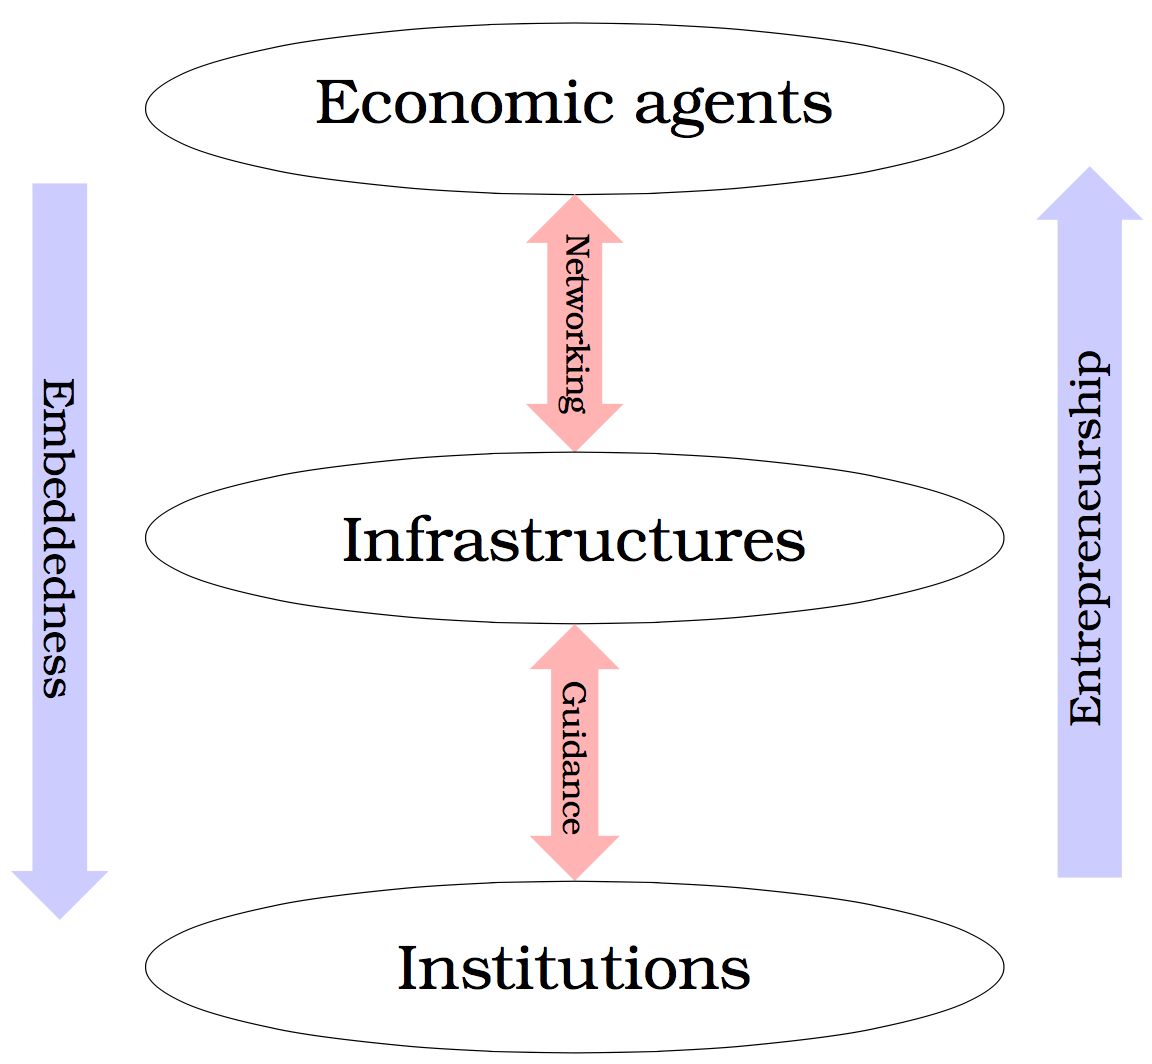
\includegraphics[scale=0.25]{imgs/structure-space.png}
\caption{Schematic representation of the socio-economic space}
\label{spacestructure}
\end{figure}

From Figure~\ref{spacestructure} we note that there exists two polar forces in the socio-economic space. The first is embeddedness; the embedding of the institutional rules into the actions and interactions of individual agents. This force---derived from the institutional structure within the socio-economic space---facilitates the formation of a steady state and adds rigidity to the actions of society. The second is represented in the form of entrepreneurship, which is the force that propagates change in the institutional framework of the economy\footnote{Interaction between economic agents and institutions through entrepreneurship is discussed in more detail in the subsequent chapters. For an excellent discussion regarding the interaction between entrepreneurs and institutions consider \citet{HenreksonSanandaji2011}.}. Society develops through entrepreneurial action and as such entrepreneurship is the antithesis to embeddedness. However, we note that feedback loops---which are a key component of any complex adaptive system---can exist between the actions of economic agents, the interaction infrastructure, and the institutions of society. Entrepreneurship can effect the governance system, which influences the embeddedness of individual agents, and can promote more entrepreneurship.

The schematic representation of the socio-economic space in Figure~\ref{spacestructure} also shows the presence of two other forces: networking and guidance. As has been mentioned above, institutions guide the actions of individual economic agents. As such, the organisational infrastructures that are formed from the actions of agents are directly determined from the institutions within the economy. Institutions guide the actions of individual agents. Networking refers to the resulting networked structure of interaction infrastructures, such that individual economic agents are positioned within a matrix of relations. Agents can arrange themselves within the matrix to positions of power, and again, this can have a feedback loop.

% Our perspective regarding a socially structured governance system is akin to John Commons position on institutional constructs. In addition to collective action of the organised variety, Commons includes disorganised custom, the laws of the state and the common law of the courts, and the patterns of conduct which a community develops for its members. Even when an individual engages in a simple exchange with another, he acts within a framework of collective law and custom, so that collective action has in fact structured the relationship. Social custom and law are perceived to be the product of these interactions. In the process of dealing with each other, bargaining, negotiating, transacting, compromising, they bend and mold their customs, modify the judicial gloss on the law, help to create the very customs which affect their economic relationships. Collective action thus controls the individual; but the individual has some power---especially in concerted effort with others---to modify the nature of collective control \citep{Hodgson2003}.

\subsection{Formalising the socio-economic space and interaction infrastructures}

The socio-economic space is represented in Figure~\ref{spacestructure} as three interacting layers: a population of economic agents; the institutions that the agents accept and trust; and the networked interaction infrastructure---the composition of the social and economic interactions that bind them. These are elements of the socio-economic space that represent the embeddedness of economic agents in a system of governance that encapsulate behavioural rules and exchange mechanisms. The space embraces relationships---consisting of \emph{bilateral economic interactions} and authority chains---or \emph{hierarchies}---formed within the socio-economic space.

\subsubsection{The socio-economic space as a mathematical concept}

A collection of economic interactions on the set of individual economic agents can therefore be regarded as a direct representation of the commonly accepted media and economic institutions that direct the interactions of the economic agents. The interaction infrastructure---including the consumer-producers that form the interactions---are the only visible aspects of the socio-economic space. This perspective of a socio-economic space allows us to make a more rigorous, and therefore more usable, mathematical definition which, by following the embeddedness hypothesis, can be represented as a set of interactions between consumer-producers.
\begin{definition}[Socio-economic space] \label{def:socioeconomicspace}
A \textbf{socio-economic space} refers to a given set of economic agents engaged in a well-described collection of general economic interactions that operate under a well-defined collection of media and institutions. 

For a given collection of media and institutions, a socio-economic space can be represented by a pair ($N, \mathcal{G}$) where $N = \{ 1, \ldots, n \}$ is a given set of economic agents and
\begin{equation}
\mathcal{G} \subset \mathcal{S}(N) \cup \mathcal{H}(N)
\end{equation}
is a given collection of \textbf{general economic interactions} on $N$, where
\begin{equation}
\mathcal{S}(N) = \{ S ~ \mid ~ S \subset N \mbox{ and } S \neq \varnothing \}
\end{equation}
is the family of non-empty coalitions in the population $N$, representing \textbf{lateral} economic interactions on $N$, and
\begin{equation}
\mathcal{H}(N) = \bigcup_{k = 2}^{\infty} N^{k}
\end{equation}
is the class of all finite ordered sequences of economic agents, representing authority chains or \textbf{hierarchical} economic interactions in $N$.
\end{definition}
The collection of all economic interactions, denoted by $\mathcal{G}$, on the set of economic agents $N$ can be regarded as an indirect representation of the commonly accepted media and economic institutions that direct the interactions of the economic agents in $N$. So, $N$ is a mathematical representation of the population and $\mathcal{G}$ is a mathematical representation of the commonly accepted media and economic institutions that guide and determine the interactions between members of the community.

The collection of economic interactions can contain a very large variety of possible economic interactions and forms of interactions. Within our set-up there are two types of economic interactions: \emph{bilateral} economic interactions and \emph{hierarchical} economic interactions. Within this monograph we focus on only one type of economic interaction: the set of simple economic interaction based on equality of the participating economic agents. These general economic interactions $S \in \mathcal{G}$ are denoted as lateral, where $S \subset N$ denotes the pair or group of interacting economic agents.

From the notion of a lateral economic interaction we derive the notion of a bilateral economic relationship. Here, an economic relationship $\{i, j\} \in \mathcal{G}$ is bilateral if the two related parties are equal partners in the generated interaction. Most trade relationships are bilateral as are partnerships in collective decision situations such as production partnerships. Structures of such bilateral relationships form a specific type of structured, collective interaction, called networks.

Although networks of bilateral economic interactions are the focus of our discussion we stress that hierarchical relationships encompass most of our regular interactions within the economy; specifically with regards interaction in a firm\footnote{For a detailed discussion of hierarchies within networked environments consider \citet{Gilles2010}.}. Hierarchical relationships are important for more developed non-primitive socio-economic spaces.

\subsubsection{The structure of interaction infrastructures}

The following definition formalises the main type of economic relationship considered. The collection of economic relationships informs the interaction infrastructure of the socio-economic space, this interaction infrastructure is termed as a network. The definition of networks below encompasses the notion of an interaction infrastructure.
\begin{definition}[Networks] \label{def:networks}
Let the tuple ($N, \mathcal{G}$) be some socio-economic space.
\begin{itemize}
	\item An economic interaction between agents $i$ and $j$, where $i,j \in N$, is \textbf{bilateral} if there is no authority present among the two economic agents constituting this relationship---and as such these two economic agents $i$ and $j$ are `equal' in the generation of the economic values through their relationship. For notational ease this bilateral economic relationship is represented as $ij \in \mathcal{G}$.

	\item A \textbf{network} is a collection of bilateral economic relationships on a given set of economic agents. Thus, a network $g$ based on $\mathcal{G}$ is given by
	    \begin{equation}
	    g \subset \{ ij \in \mathcal{G} ~ \mid ~ i,j \in N \} .
	    \end{equation}

	\item A \textbf{complete network} is a network in which all economic agents are connected to each other by some bilateral economic relationship. Thus, a network $g$ is complete if and only if
	    \begin{equation}
	    g = \left\{ ij ~ \mid ~ i,j \in N \mbox{ and } i \neq j \right\} .
	    \end{equation}
	We denote a complete network on $N$ by $g_{N}$.

	\item An \textbf{empty network} is a network in which there exists no economic interactions between the population of $N$ consumer-producers~\footnote{An empty network is a representation of a monadic economy discussed as given in Definition~\ref{def:autarkyproblem}}. Formally, a network $g$ is empty if and only if $g = \varnothing$.
\end{itemize}
\end{definition}
A network is a derived notion such that the structure is part of the collection $\mathcal{G}$. Models that partition the demand and supply of a trade situation suggests that bilateral interaction between agents are conducted in a bipartite manner such that one side of the interaction is designated as the supply-side and the other side is designated as the demand-side. Models that partition the demand and supply of a trade situation are described in the form of a bipartite network.
\begin{definition}[Bipartite networks] \label{def:bipartiteNetworks}
A network $g$ on a set of economic agents is \textbf{bipartite} if there are two disjoint coalitions $N_{S} \subset N$ and $N_{D} \subset N$ with $N_{S} \cap N_{D} = \varnothing$ such that $ij \in g$ implies that $i \in N_{S}$ and $j \in N_{D}$. Hence, the only feasible economic relations are between a member of $S$ and a member of $D$. Naturally, $S$ and $D$ refer to the supply and demand side in the bipartite network $g$.

\noindent A bipartite network $g$ is \textbf{complete} if $g = N_{S} \otimes N_{D} = \{ ij ~ | ~ i \in N_{S} \mbox{ and } j \in N_{D} \}$.

\noindent A bipartite network $g$ is \textbf{minimally connected} if every consumer-producer in $N$ is engaged exactly one economic interaction each.
\end{definition}
By allowing there to exist a dichotomy between the demand and the supply-side of economic interaction markets of bilateral interactions are represented as a bipartite network. These models partition a set of economic agents into a set of consumers (demand) on one side and a set of producers (supply) who produce some output on the other. Given some set of valuations for the producers output, consumers form trade relationships with suppliers given the actions of all other consumers in the market and the price levels that naturally emerge from the demand and supply for these tradable outputs. These discussions introduce the notions of perfect competition, monopoly, and traders within a bipartite network.

We do not draw such a strict dichotomy between the consumption and production of agents. Instead, as noted in Axiom~\ref{dichotomyhype}, we structure economic agents as both consumers and producers endowed with both consumptive properties and production possibilities. The consequence is a network that can take forms that are potentially divorced from the bipartite structure. Representing economic agents as consumer-producers can naturally lead to the formation of irregular and elongated economic networks. Small-world and scale-free networks can also arise depending on the exchange mechanism imposed. Within these structures individual agents have differentiated positions. These positional attributes can be distributed in an unequal fashion across the network leading to unique opportunities and constraints for agents that possess certain positions in the network.

For completeness we note that another common structure found in both theory and reality is a \emph{star network}, which is referred to in later discussions of network centrality.
\begin{definition}[Star network] \label{def:starNetwork}
A network $g \subset G_{N}$ on $N$ is a \textbf{star} if there exists some consumer-producer $h \in N$ such that
\begin{equation}
g = \left\{ ih ~ \mid ~ i \in N \mbox{ and } i \neq h \right\}.
\end{equation}
Therefore consumer-producer $h$ is at the center of the star.
\end{definition}
This section has provided some structure to the relational theory in two ways. First, we provided an environmental concept that acts to encapsulate the fundamental notions of the relational perspective: this was defined in terms of the socio-economic space. Second, we added structure to the socio-economic space by defining it in mathematical terminology. The insights discussed in this section help in the formal discussion later in the monograph.

The socio-economic space is a dynamic concept. As noted by the schematic representation of the socio-economic space in Figure~\ref{spacestructure} this dynamism is triggered by pressures that derive from entrepreneurial activities. We elaborate on the \emph{states} of the socio-economic space and the mechanism of development through entrepreneurial activity.

\section{States of the socio-economic space}

Particular economic states can be identified through the characteristics of the governance system and interaction infrastructures, which economic agents are ultimately embedded and operate within. At this point we do not comment on how one economic state transitions to another other, but instead focus on potential states that can exist. It is unlikely that the space merely tips from one state to the other; it may indeed be a gradual phase transition of self-reinforcing institutions that are punctuated by institutional and network alternations, which are reflected in notable changes in certain aspects of the governance system.

\subsection{Pure states of the socio-economic space}

A `pure' economic state is one that can only be achieved at a theoretical level. Pure economic states will not exist in reality. Here we provide two pure states of the socio-economic space. The first state---\emph{the state of nature}---describes a relatively primitive socio-economic space whereby institutions and systems of governance exist to obstruct the formation of functional social and economic interactions leading to a difficulty in the generation of wealth throughout the economy. This is not to say that institutions do not exist at all, but the institutions that do exist are either too costly to facilitate exchange or they are formed specifically to hinder the formation of economic relationships between agents. We note that the state of nature can exist as a manufactured state to, for example, suppress an underclass. The second state---\emph{the trustified economy}---refers to a socio-economic space in which corporations have a significant impact on the development of the economy. Specifically the role of competition, the development of new firms, and new the exploitation of new entrepreneurial opportunities are not the driver of change; but pre-existing companies monopolise the development of the governance system. Note that these states should only be considered as theoretical extremes, not a realistic indication of the socio-economic space.

\subsubsection{The state of nature}

In \emph{Leviathan} \citet{Hobbes1651} discusses the emergence of monarchs and governing bodies through the formation of a social contract. According to Hobbes a civilisation could raise itself from a `state of nature' to the formation of functional relationships ultimately governed by absolute government in the form of a monarch. From this structure of rule and enforcement, built on the basis of social contract, civil society could flourish.

The state of nature considered by Hobbes was characterised by the non-existence of, or presence of dysfunctional, social and economic relationships between individual agents. According to Hobbes men are born equally; from this equality, and the inherent violence of man, Hobbes claimed that this would lead to wars and conflict among men so that, ``during the time men live without a common power to keep them all in awe, they are in that condition which is called warre; and such a warre as is of every man against every man''. During this state every person has a liberty to to anything one perceives as necessary for preserving one's own life; and thus life would be, ``solitary, poor, nasty, brutish, and short''. This is the war of all against all whereby cooperation and the presence of functional, wealth-generating social and economic interactions are non-existent.

The essence of this economic state is developed from Thomas Hobbes' initial depiction of the state of nature. However, we do not assume the absence of systems of governance, but instead consider a socio-economic space comprised of dysfunctional systems of governance and therefore the formation of economic interactions between agents is costly. These may be imposed from a top-down manner from an oppressive elite. This results in a \emph{monadic} economy whereby all economic agents act autarkically thus consuming their own output only. Under the state of nature the organisation of society is in its simplest form. In line with Hobbes, the state of nature requires no trust between agents and institutions; and, as such, welfare is at its most primitive.

We do not specifically advocate that this state has ever existed or can exist. The formation of simple institution such as signalling or emotional gesture in which to base simple relationships is also an evolved part of the human species. We are social creatures, and as such, social relations are fundamental and this state of nature is purely theoretical. Alternatively, it can be likely that institutions and systems of governance exist but the costs of using them or even understanding them are too high. In this case the interaction inefficiency is excessive and the formation of social and economic relationships suffer. Given high levels of interaction inefficiency an economic state may revert to a state close to that of the state of nature or monadic economy. As a consequence all economic agents earn near subsistence levels of utility. 

The ultimate claim of this state of nature is that the governance systems are deficient for the society to form structured relations with each other. This deterioration of social and economic capital degrades the structure and development of the governance system. \citet{Granovetter1992} noted that a lack of trust and social capital within society would stifle the creation and development of institutions and organisational patterns of production. In stipulating the construction of institutions \citet[p.~7]{Granovetter1992}, ``economic institutions do not emerge automatically in response to economic needs. Rather,they are constructed by individuals whose action is both facilitated and constrained by the structure and resources available in social networks in which they are embedded.'' He elaborates by providing a discussion of how lesser-developed economies are unable to form recognised firms and elaborate exchange networks. This is also discussed later by \citet{deSoto2001} and \citet{AcemogluRobinson2012}. The state of nature is a more extreme version of the social and economic environment discussed by these authors; the systems of governance are sufficiently dysfunctional such that social and economic relationships are nonexistent, and each agent effectively operates at substance levels.

% This state of the socio-economic space may have equally been attributed to Malthus due to the consequence of the `Malthusian trap'. In \emph{An Essay on the Principle of Population} Thomas Malthus (1798) discusses how without war, disease, or natural disaster the growth rate of the worlds population was exponential whilst the growth of the worlds food-stock was arithmetical. Therefore, according to Malthus' logic, the growing population size would eventually outstrip the food supply leading to the eradication of society as a whole unless `preventative checks' and `positive checks' were applied to regulate the population against the food supply. In Malthus' terms a preventative check was one that was socially developed and would thus lead to a relative stagnation of the population. These preventative checks included abstinence and marriage restrictions. A positive check was a naturally occurring phenomena that would balance the demand and supply of food. Specifically a positive check included starvation and war.

% The state of the world proposed by Malthus leads to the emergence of a so-called Malthusian trap which, according to many economists (Fogel, 2004; Clark, 2007), occurred for much of human history. A Mathusian trap exists when the per capita income within an economy is largely stagnant due to the emergence of new technology leading to population growth as opposed to improvements in the standard of living. Such a phenomenon suggests that over time per capita income does not improve, technology development is slow and largely ineffective, therefore the state of the world is stagnant as economic agents earn subsistence levels of utility; as can be seen in the Hobbesian economy.

\subsubsection{The trustified economy}

The trustified economy is characterised by the centralisation of influential power of the governance system to platforms, or corporations. This power is derived from increased bargaining power with the \emph{de jure} elite due to their economic resources and from their ability to fund research in innovation. Development is monopolised by the power of \emph{de facto} elites.

Whilst witnessing the rise of large corporations largely supported by trusts---such as Standard Oil, J.P. Morgan \& Co. and General Electric---Joseph Schumpeter first discussed the notion of a trustified economy, or more precisely ``trustified'' capitalism as opposed to ``competitive'' capitalism, and hypothesise a trend of economic progress towards this trustified state. Within this trustified state \citet[p.~384]{Schumpeter1928} claimed that, ``[i]nnovation is... not any more embodied \emph{typically} in new firms, but goes on, within the big units now existing, largely independently of individual persons. It meets with much less friction, as failure in any particular case loses its dangers, and tends to be carried out as a matter of course on the advice of specialists. Conscious policy towards demand and taking a long-time view towards investment becomes possible''. Development in the trustified state becomes `automated', increasingly impersonal and decreasingly a matter of leadership and initiative.

The trustified state suggests that the waves of \emph{Creative Destruction} are diluted---or, in an extreme sense, non-existent---compared to competitive capitalism in which new firms enter the economy and displace old obsolete firms. Innovation in competitive capitalism is embodied by entrepreneurs and the foundation of new firms, ``... improvement is forced on the whole branch by the processes of underselling and of withdrawing from them their means of production, workmen and so on shifting to the new firms; all of which not only means a large amount of disturbance as an incident, but is also effective in bringing about the result, and to change `internal' economies into `external' ones, only as far as it means disturbance'' \citet[p.~384]{Schumpeter1928}. This is different in a trustified state of capitalism. Within a trustified state there exists little disruption from entrepreneurs or groups of entrepreneurs through the provision of new firms, new innovative outputs, new production processes, new socio-economic roles, or new political agenda. Instead a paradox arises whereby innovation becomes frequent, predictable and, as a consequence, tedious; doing little to improve society's welfare or even disequilibriate the economy.

Moreover, according to Schumpeter, the trustified state encourages more focus on the automation of processes and, although the division of labour deepens and new socio-economic roles born, the effect is an alienation of individuals and an enlarged separation between the actions of individuals and their overall outputs. This is a typical Marxian conclusion regarding the evolution of capitalism, later repeated by \citet[p.~77]{Milgram1973}: ``....as soon as there was a division of labour things changed. Beyond a certain point, the breaking up of society into people carrying out a narrow and very special jobs takes away from the human quality of work and life. A person does not get to see the whole situation but only a small part of it, and is thus unable to act without come kind of overall direction. He yields to authority but in doing so is alienated from this own actions.'' In fact, Schumpeter's and Marx's ultimate conclusion for the state of capitalism are not dissimilar. In his concluding sentence \citet[p.~386]{Schumpeter1928} hypothesised that, ``[c]apitalism, whilst economically stable, and even gaining in stability, creates, by rationalising the human mind, a mentality and a style of life incompatible with its own fundamental conditions, motives and social institutions, and will be changed, although not by economic necessity and probably even at some sacrifice of economic welfare, into an order of things which it will be merely matter of taste and terminology to call Socialism or not.'' The trustified state was, to Schumpeter, the final stage of capitalism.

The ultimate conclusion of Schumpeter is stark and debatable---a debate that is certainly beyond the scope of this monograph. Instead, our notion of the trustified economy utilises Schumpeter's initial claim regarding the influence of large firms to monopolise innovation, and therefore motivate a change to the governance system and propagate the development or regression of the socio-economic space. With respect to the neoliberal economy less emphasis is placed on individual entrepreneurs and Government to direct development, and more emphasis is placed on pre-existing firms and sources of financial capital. The socio-economic space is therefore characterised by increasingly hierarchical relations within the context of sprawling production organisations.

There are three concluding points to note. First, within the trustified state the action of entrepreneurship is completely replaced by the action of management who exist within transnational firms. Second, is that the trustified economy is only considered as a `theoretical extreme', in that it is unlikely that individual or coalitions of entrepreneurs will become completely redundant and the the supply of new firms to the economy will stop. Furthermore, it is unlikely that the role of government be displaced by corporations and that elected individuals will relinquish their powers to affect the institutions of the governance system. Second, role-building costs and interaction inefficiencies are considered to be reduced due to the presence of more structured institutional environments.

% \subsubsection{The Marxian economy}

% Need discussion on `theoretical communism' here!

\subsection{Representative economic states}

By extending the theoretical extremes of the pure economic states above we provide a typology regarding all more realistic, or \emph{representative}, economic states of the socio-economic space. We specifically provide insight regarding three of these states that have been recorded over time. Each state signifies a notable difference in the governance system and the interaction infrastructures present in the socio-economic space. 

As a socio-economic space develops we tend to see a more structured vertical division of labour and a deeper division of labour with objective socio-economic roles organised by hierarchical relationships. Therefore, in order of development these representative economic states are: (1) the Platonian economy; (2) the incorporated economy; and (3) the platform economy.

\subsubsection{The Platonian economy}

The Platonian economy is perceived as a `human' or `organic' economy within which the source of wealth emerges through social organisation founded specifically through human ability, specialisation, and limited innovation. It is the ability for humans to organise social production situations within a networked market that is the source of all wealth in this economic state. The organisation of economic activity can only be done on the basis of a controlled and ordered society; specifically ordered through the creation of accepted primitive rules of exchange, well-defined socio-economic roles, and behavioural norms. Thus, governance systems exist to form functional relationships.

Within a Platonian economy agents are assumed to be equal parts when interacting and cooperating with each other. Within predominantly tightly-knit networks relatively small communities tend to favour simplistic conventions of trade, thus facilitating egalitarianism and fairness; no economic agent tends to be more powerful than the rest meaning that hierarchy is primitive. However, positional power may emerge from the socio-economic roles that individuals specialise in.

This type of organisation provides the basis for specialisation and the creation of socio-economic roles completely dependent on an individuals' abilities and on the actions and specialisations of the local society. Within this type of economy, socio-economic roles are primitive, which means that an individuals' specialisation will be purely dependent upon their local socio-economic environment which includes the current organisation and specialisations of those in society, the resource base, and the technology that is apparent within the economy. The resulting coordinated specialisation of an individual results in a higher productivity and wealth creation in society. In other words, the human ability to coordinate allows for the access to increased productivity through specialisation as well as for the realisation of the resulting gains from coordinated social production.

We denote this primitive state of the socio-economic space as the Platonian economy due to the time and context of Plato's writing, which, as mentioned in our discussion of the division of labour in Chapter~\ref{ch:relationalperspective}, focuses primarily on the horizontal division of labour. In his writings of city formation he claims that the majority of economic interactions exist within a market context with a horizontal division of labour. This interaction is outside of the environment of a well-defined organisation such as firms or corporations, and thus a vertical division of labour. During his time of writing corporations did not exist and it is unlikely that firms, even in the most primitive sense of the word, existed to a notable extent. More centralised and organised production techniques are the feature of a more developed socio-economic space. These indeed play a prominent role in incorporated and platform economic states.

The human species recognised early that individuals, with the ability to specialise in a variety of productive tasks, can be socially organised to achieve a society that generates collective economic wealth. This social organisation is subject to not only increasing returns to specialisation, but when working together, increasing returns to scale. This social organisation is usually called the `social division of labour' and forms the foundation of any human society. The organisation of the Platonian economy refers to the division of specialised tasks among individuals within a human community. It refers to the social organisation of a community to achieve a collective social economy that is collectively subject to increasing returns to scale in its productive abilities. Within a social division of labour individual economic agents assume individualised production tasks. This requires that individuals perform tasks that are recognisable by all members of the society as socially acceptable and economically viable.

This social recognition involves two elements. First, the social recognition of an economic, productive task requires that the task is performed with socially recognised inputs and outputs. Thus, each task within a social division of labour concerns the conversion of socially recognised and specified inputs into socially identifiable and measurable outputs. Second, the social division of labour is only functional as a social organisation if the generated socially recognised outputs can be distributed among the members of the society in a socially recognised fashion. In economic terms, the generated outputs are publicly exchangeable with outputs generated by other specialised individuals. Such a public exchange can only occur through socially recognised exchange mechanisms.

These two elements leads to the conclusion that a social division of labour requires a supportive governance system. As mentioned previously, all economic interaction has to be considered to be embedded in an appropriate social governance system. The embeddedness of economic interaction within a governance system is fundamental to our understanding of the organic Platonian social economy. We can loop this back onto the interpretation and clarification of the social division of labour as a system in which individual production tasks are combined with economic exchange. Indeed, the organisation of social economy is formed as a social division of labour in which individuals execute specialised productive tasks and exchange the resulting outputs from these tasks through socially recognised exchange mechanisms.

The nature of the horizontal and vertical social division of labour is that tasks are performed in a structured sequence. This allows the production of relatively complex consumption goods: such goods are realised through a sequence of intermediate stages performed by distinct specialised individuals. The Platonian economy allows for this and this form of exchange through intermediaries is used throughout Chapters~\ref{ch:criticalnodes} and~\ref{ch:blocks}. Under this structured sequence of exchange economic agents can fully utilise their relational attributes.

Platonian economic states can be characterised by high role-bulding costs. Within primitive environments agents engage in a process of adaptive specialisation due to the absence---or relative deficiency---of more structured educational institutions. In more advanced Platonian economies roles can be built through apprentice and kinship relations, therefore agents will dictate the specialisation of individual economic agents. Moreover, patrilineality and family ties can also play a distinct role. We note the importance of these institutions to support role-building and specialisation with respect to the case of Renaissance Florence in Chapter~\ref{ch:entrepreneurship}. \citet{NorthWallis2006} suggest that in primitive societies the identities of individual agents were based prominently on social roles as opposed to the economic context of their roles. As such, the identity of individuals was based more on the characteristics and patrilineal ties of the individual as opposed to the economic position and ties of the individuals. Specifically, the reputation and perhaps the role of the individual would have depended more on the family of the individual as opposed to the socio-economic role that the individual autonomously specialises into. As our society has developed, and we require interacting with a greater wealth of individuals, more emphasis has been placed on the importance of socio-economic roles and related action-sets as opposed to more personal identities.

We conclude that the social division of labour results into well-structured social production chains, naturally resulting into the conclusion that the economy is founded on a complex network structure. These complex networks are initially shown in the Platonian economy. Again, we generalise this insight beyond the constrained view of the social division of labour and apply this to any human economic interaction.

\subsubsection{The incorporated economy}

A socio-economic space can include hierarchical relations as well as purely economic exchange relations. We contend that as the socio-economic space develops the economic interactions and relationships that emerge within it become progressively hierarchical and the governance system, including the socio-economic roles, become more structured. The Platonian economy omits the existence of ``hierarchical production organisations''. These organisations---generally regarded as firms or corporations---internalise relationships between specialised individuals through an authority guidance structure. This organisational form clearly delineates incentives and makes the guidance of decisions and tasks more transparent and effective than through the more organic horizontal division of labour. Instead of individuals being guided by external forces, they are subordinated within an authority structure. The result is the existence and fruition of a vertical division of labour based on some incomplete labour contract.

The introduction of hierarchical production organisation requires the development of a more structured governance system, typically through entrepreneurial effort, and can lead to the generation of a deeper division of labour with more automated socio-economic roles. The horizontal division of labour in the Platonian economy suggests that all economic exchange is conducted within a network by a set of equal socio-economic agents in terms of their authority. Typical interaction inefficiencies exist with regards the existence of transaction costs \'{a} la \citet{Coase1937} and \citet{Williamson1971, Williamson1975, Williamson1979}. From this perspective we can see that as interaction inefficiencies increase in the exchange networks a horizontal division of labour is substituted for a vertical division of labour and the exchange networks are shortened accordingly.

The incorporated economy illustrates the benefits of increasing returns to specialisation from the automatisation and deepening of the division of labour within a coordinated and centralised environment. Hierarchical production organisations within this state are considered to be the workhorse regarding the generation of wealth throughout the socio-economic space. Therefore, organisation within an incorporated economy deviates from a Platonian economy in this regard. Specifically, within an incorporated economy the economic decision-making by individual agents is more centralised within a hierarchical structure, and therefore the majority of strategic decision-making is done by `principals' and subsequently carried out by `agents'. Relationships within a firm are incomplete in the sense that the principle usually has insufficient ability and information to precisely assess the task and performance of the agent. This is due to the specialised nature of the tasks done by these individuals within the authority structure. As such, traditional principal-agent relationships based on information asymmetries arise as the majority of economic agents suffer from a loss of autonomy \citep{JensenMeckling1976, Eisenhardt1989}.

The consequence of the formation of hierarchical production organisations is that decision-making is more interdependent and the interactions that exist between agents are embedded within a well-defined, structured and accepted governance system. Moreover, socio-economic roles become more structured and automated, which facilitates the invention of technologies to substitute and complement existing divisions of labour. The incorporated economy is the first economic state in which the social division of labour---which is the only form of the division of labour in the Platonian economy---is rivalled with a division of labour within the firm as explicitly discussed by Adam Smith. Thus, the incorporated economy is the first state to introduce both bilateral and hierarchical economic interaction: the Platonian economy was restricted the assessment of bilateral economic interaction only. Standard transaction cost and contract theory \citep{Cheung1983, AghionHolden2011} regarding the establishment of the firm against economic interaction within a market environment apply here.

As noted by Coase, inefficiencies naturally exist within both firm and market interactions; however, the establishment of firms aims to minimise these. This suggests that the interaction inefficiency of an incorporated economy is high, but lower than the inefficiency within a Platonian economy. The institutions are relatively well-defined, but are still costly to use. These costs depend on how well defined they are, and how available more formal institution are to society as a whole. The government has some role to play in the maintenance of these institutional structures.

\subsubsection{The platform economy}

A platform economy is one that is most closely related to that of a contemporary developed economy. Under this setting the notion of a hierarchical production organisation is further developed from the incorporated perspective---considered as firms and corporations---through the formation of elongated hierarchical relationships and the increasing returns from a deepened division of labour, economies of scale, and economies of scope. Developed hierarchical production organisations have more prominence and power in a platform economy than in an incorporated economy; however their structure and scope is larger. As opposed to witnessing hierarchical economic interaction within the context of a firm or corporation we now see this interaction within vaster and more complex structures that we term as a \emph{platform}.
\begin{definition}[Platform] \label{def:platform}
An economic agent or hierarchical production organisation is a \textbf{platform} if it exists in multiple aspects of a socio-economic space and facilitates interaction between aspects between these for other economic agents and hierarchical production organisations.
\end{definition}
A platform is an economic agent or hierarchical production organisation that, due to its position and multivocality, has an ability to enable economic interaction between aspects and can potentially extract from other economic agents by brokering relations. Thus, a platform can both \emph{enable} the formation of economic interactions and can \emph{extract} the wealth generated from these interactions. As a consequence, a platform is a hierarchical production organisation that operates within different aspects of a socio-economic space and as such is able to monopolise interaction both between and potentially within those aspects. We could consider a platform as a middleman that operates in many aspects of a socio-economic space---combining multiple socio-economic roles---and as such monopolises exchange between those those aspects.

In conventional syntax we may associate a platform with an uncontested transnational corporation or conglomerate which, by virtue of their function and place in the economy, operates in multiple sectors and has an ability to connect those sectors together. This may be done through the facilitation of economic interactions between those sectors---much like a `market-maker'---or alternatively done by producing an intermediary output that has function within multiple sectors. The defining feature is that platforms have power in multiple sectors of an economy and can use that to their advantage.

The deepening of the division of labour and the subsequent automatisation of roles, first introduced in the incorporated economy, is recorded to a greater extent within platforms. Production processes carried out by technology leads to considerable depersonalisation and redundancy of the `human' division of labour. The consequence is two-fold: first, the redistribution of the population to more productive socio-economic roles; and second, is a redistribution of wealth to those more productive roles. Thus, any friction in terms of role-building costs may lead to an unequal distribution of wealth and utility within society.

\medskip\noindent The assessment of economic states implies that the socio-economic space is a dynamic concept that develops over time. Moreover, an inference from the assessment of different socio-economic states is that the development of the socio-economic space---the context of the roles and interactions, the institutional structures, and the elements of the governance system---brings with it a progressively hierarchical society. More complex structures arise and are built upon as the space of interactions evolves from a monadic state of nature, to a primitive Platonian economy with general economic interactions, to an industrialised incorporated economy with hierarchical production organisations, to a platform economy, and finally to a trustified economy. 

The evolution of the socio-economic space also illustrates tendency toward a wider array of well-defined socio-economic roles, a more distinctive presence of automated `non-human' or `inorganic' socio-economic roles, and more sophisticated institutionalised structures for supporting a deepened division of labour. The driving force of this development is the actions of entrepreneurship. Below we introduce the notion of entrepreneurship within the context of growth and development of the socio-economic space.

\section{Growth, development, and the entrepreneur}
\label{subsec:growthdev}

Figure~\ref{spacestructure} introduces a set of important forces within the socio-economic space. We have already discussed the forces of embeddedness with respect to socio-economic roles, networking with respect to formation and structure of interaction infrastructures, and guidance with respect to institutions within the governance system the guide interaction and behaviours. Our discussion thus far has, however, been deficient with respect to the force of entrepreneurship, which acts to influence a change within the layers of the socio-economic space. The act of entrepreneurship is closely related to the development of the socio-economic space, and its transition from one state to another. Importantly, it is an action that impacts all three layers of the socio-economic space: the population of economic agents, the structure of the interaction networks, and the institutions within the socio-economic space.

\subsection{Distinguishing growth and development}

The growth and development of the socio-economic space are considered as two distinct but related processes. Both lead to similar outcomes---the improvement or redistribution of aggregate utility across the population of economic agents---however, the distinction between them is important; particularly for the discussion of the entrepreneur and entrepreneurship. Their distinction can be highlighted in the set of definitions below.
\begin{definition}[Growth and development] \label{def:growthanddevelopment}
A socio-economic space can grow and develop. These are two distinct notions.
\begin{itemize}
	\item The \textbf{growth} of a socio-economic space refers to a change in some fundamental or pre-existing parameters that define the socio-economic space such that the aggregate utility of all economic agents increases.

	\item The \textbf{development} of a socio-economic space refers to a productive change in the elements of the governance system such that the new institutional mechanisms produces an increase in aggregate utility.
\end{itemize}
\end{definition}
The growth of a socio-economic space corresponds to changes in parameters that describe the economic agents, the extent of their actions and specialisation, and the size of the space they interact in. These parameters include the size of the population of economic agents, the cost of interaction and the size of the interaction inefficiency, and the extent of their individual production technologies. Improving changes in these parameters leads to an increase in aggregate utility, however the structure of the interaction infrastructure and the exchange conventions remain constant. Importantly, the composition of the governance system remains constant given the growth of the socio-economic space.

The development of a socio-economic space corresponds to a direct alteration in the composition of the governance system. These alterations include the creation of a new socio-economic role, socially recognisable output, trading mechanism, or interaction infrastructure. Improving changes can lead to the extension of the division of labour or organisation of society given the rule sets provided by the institutional framework.

Despite differences in definition, the notions of growth and development are related such that the development of the socio-economic space through, say, the deepening of the division of labour can lead to the growth of the socio-economic space through the improvement of production technologies or the facilitation of previously unconnected economic agents to exchange with one another. In this way the notions of growth and development interact with one another: a socio-economic space can go through a relatively slow process of growth and then a period of development which prompts a punctuated change in the equilibrium organisation of society; this itself induces a period of growth.

% % % Can be brought to the Appendix

\subsubsection{Decline, regression, and The Edge of Chaos}

Equally as interesting are the notions contrary to the growth and development of the socio-economic space: namely \emph{decline} and \emph{regression}. The decline of a socio-economic space---as considered the opposite of growth---refers to a change in some fundamental parameters that induce a decline of aggregate utility of all economic agents. An example of this decline can be a reduction of an economy's population leading to a reduction in its Gross Domestic Product\footnote{The fall in Japan's Gross Domestic Product since 2010 can be illustrative of the decline of a socio-economic space in the form of a population decline \citep{Economist2014}. However, some see it as a consequence of more fundamental Japanese cultural norms backed by formal institution \citep{West2011}.} or can be a reduction of productivity due to a deterioration of an economy's capital base. Again, the decline of a socio-economic space, much like its growth, is typically classified as a relatively slow process.

On the other hand, the regression of a socio-economic space---as considered the opposite of development---refers to a destructive alteration of the governance system which induces a fall in aggregate utility across the population of economic agents. Examples of this include the adoption of a behavioural or cultural norm that reduces productivity, the deterioration of educational institutions, or the presence of ill-defined or perverse institutions that do not facilitate functional wealth-generating economic interactions\footnote{An appropriate example could be the recent global financial crisis and subsequent Sovereign Debt crisis. Many see this crisis as a symptom of an institutional malaise \citep{Crotty2009, Ferguson2014} as well as a fundamental outcome of the economics discipline itself \citep{Hodgson2008, Hodgson2009, Krugman2009}.}. Much in the same way as development, the regression of a socio-economic space can be a punctuated event.

The theory of punctuated equilibrium is extremely important. The economy as a complex adaptive system can gravitate towards a so-called ``Edge of Chaos'' : the fertile ground between too much order and too much randomness; a concept attributed to Christopher \citet{Langton1990}, and subsequently popularised in finance literature by Nassim \citet{Taleb2007, Taleb2013}. Self-organising systems of interdependent parts progressively optimise to a certain point whereby any deviation will cause the system to malfunction and collapse. This edge of chaos terminology can be used to describe the institutional structure and the resulting dynamics of economies. In the final chapter of \emph{Civilisation}, Niall \citet{Ferguson2011} argues that empires---the Roman, the British, the French---experienced a punctuated collapse. This is an argument also discussed by Jared \citet{Diamond2011}. In their evolutionary strive for efficiency they develop networks and institutions that are highly interdependent, meaning that if one network or institution were to collapse the economy as a whole could tip into failure. In the strive for efficiency a socio-economic space can become highly prone to failure. Such an observation fits well with the potential unraveling of interdependent forms of trust.

% % % 

\subsection{Entrepreneurship and the entrepreneurial function}
\label{sec:entrepreneurship}

The development of the socio-economic space is propagated by the actions of the \emph{entrepreneur}. It is the entrepreneur---through the process of \emph{entrepreneurship}---that facilitates the evolution of the socio-economic space through the modification of the elements of the governance system and, as a consequence, alters the welfare of economic agents that use the governance system to interact. 

The entrepreneur is essential in the transition and maintenance of a certain type of economy, and whose function gathers importance as the socio-economic space develops. For example, in the state of nature entrepreneurship and the entrepreneurial function is absent due to the dysfunctional governance system and the non-existence of social and economic relationships. On the other hand, in a trustified economy entrepreneurship is common and routinised by non-personal economic agents. In the trustified economy changes to the governance system are regular and subject to change from one time period to the next. The development of entrepreneurial models built with the intention of encompassing institutional and social aspects are of paramount importance as their ultimate role will indeed depend on the structure of the socio-economic environment which they operate in \citep{AldrichMartinez2007}.

The schematic in Figure~\ref{spacestructure} notes that the socio-economic space can be partitioned into three distinct layers, namely: the population of economic agents that interact within the socio-economic space; the infrastructures that are created from their interaction; and the institutions that reflect and enforce the rules of interaction. We note that the act of entrepreneurship operates in all layers of the socio-economic space described. Entrepreneurship can, for example, lead to the provision of new products and processes that increase the production sets of a population of economic agents, provide a new architecture to existing interaction infrastructures, or lead to the modification or introduction of new institutional structures. We provide definition to these concepts below.

\subsubsection{Defining entrepreneurship and the entrepreneurial function}
\label{definingentrepreneurship}

An entrepreneur refers to an economic agent that engages in entrepreneurship, a set of actions that refer to a higher form of adaptive specialisation within a given socio-economic space.  Entrepreneurship is an action or set of actions taken by individual economic agents that go beyond the choice space defined and imposed through the prevailing governance system of the economy. This specialisation affects two categories of the socio-economic space: the governance system itself, and its networked interaction infrastructure. All actions that result into new developments in the governance structure or in the trade infrastructure underlying the economy can be regarded as ``subjective innovation'', since these entrepreneurial actions---and subsequent innovations---usually derive from actions already exhibited by individuals within a given socio-economic space.

The \emph{entrepreneurial function} is a weaker notion than that of entrepreneurship and should be considered separately. Both are considered as actions that impact the socio-economic space in some way, but the most notable difference between entrepreneurship and the entrepreneurial function is that the latter is not necessarily carried out by entrepreneur and as such affects the structure of the socio-economic space in a more minor way. Indeed, the entrepreneurial function, as distinct from entrepreneurship, is the slight modification of a given socio-economic role for operation in a given context or the formation of new economic interactions and relationships with a given socio-economic role and recognisable output. The entrepreneurial function can, and is, conducted by all economic agents of a given population. It does not directly lead to the deepening of the division of labour, the formation of new socio-economic roles, new outputs and technologies, a reformation of the socio-economic space, or new influential positions in the network, and thus does not spur development of the socio-economic space. However, the economic agent can spur growth through the process of the entrepreneurial function.

This discussion of the entrepreneur and the entrepreneurial function allows us to make a definition on which to expand upon throughout the monograph.
\begin{definition}[Entrepreneurship and the entrepreneurial function] \label{def:entrepreneur}
Consider a socio-economic space with a population of economic agents and a governance system of socio-economic institutions.
\begin{itemize}
\item An \textbf{entrepreneur} is an economic agent who, through her actions, engages in entrepreneurship.
\item \textbf{Entrepreneurship} refers to actions that modify in a major way elements of the governance system and the underlying interaction infrastructure in the socio-economic space, thus directly or indirectly impacting the population of the socio-economic space.
\item The \textbf{entrepreneurial function} refers to actions that modify in a minor way elements of the socio-economic space, thus directly impacting the individual economic agent and her local environment.
\end{itemize}
\end{definition}
For clarity we note two main differences between entrepreneurship and the entrepreneurial function from the definition above. These two differences can be distinguished as `scale' and `creativity'. With regards scale we note that entrepreneurship is conducted at a larger scale than the entrepreneurial function. Indeed, the impact of entrepreneurship leads to a change in the structure of the governance system that is used by all agents within the socio-economic space; therefore the process of entrepreneurship directly impacts all agents of the socio-economic space. This is not the case with regards the entrepreneurial function. The entrepreneurial function directly impacts the economic agent conducting it and her connections only. Indeed, it may impact others in the population indirectly, but the effects of the entrepreneurial function are directed and do not lead to a change in the elements of the governance system.

With regards creativity we note that entrepreneurship is inherently innovative and, as such, all subsequent changes to the governance system are new. The creativity of the entrepreneurial function is reflected in the formation of new socio-economic roles, new outputs, new mechanisms of exchange, and new interaction architectures, that are subsequently embedded in the socio-economic space. The creativity of the entrepreneurial function is limited, and thus does not generate anything inherently new in the economy. This distinction with regards the innovativeness of the entrepreneur is important when making a general distinction between the two actions.

Whereas entrepreneurship is the main workhorse for the development of the socio-economic space, the entrepreneurial function along with external parameters such as population growth are the main forces of the growth of the socio-economic space. The evolutionary nature of development and the entrepreneurial function characterised by punctuated changes in the socio-economic space. This notion is based on an initial discussion by \citet{GillesLazarovaRuys2006} who propose the formation of a stable socio-economic space based on a social division of labour of objective socio-economic roles as initially emerging from a state of chaos.

This definition of entrepreneurship is strong relative to the existing literature. Within the relational perspective, entrepreneurship refers to more than self-employment---as is the typical indicator for many analyses of the topic \citep{EvansJovanovic1989, Lazear2004, CagettiNardi2009, SanandajiLeeson2013}---but must include actions that alter the governance system of the economy in a substantial way. As a consequence the notion of entrepreneurship coincides with Schumpeter's perception of the entrepreneur providing a disequilibrating force to the economy. Our point of departure is to claim that the entrepreneur should not be perceived as simply an agent that interacts within a market context; but can actively disequilibrate a socio-economic space through influencing a change to the governance system. Further still, and perhaps most importantly, we accept that entrepreneurship leads to the extension of the division of labour and the development of new socio-economic roles. As a consequence new positions emerge in the socio-economic space and entrepreneurial individuals can build on those positions and potentially earn rents and profits from doing so\footnote{A more elaborate discussion of the socio-economic space is left until the subsequent chapters. The next chapter provides an overview regarding the established theories entrepreneurship and how the relational fits with these established theories.}.

\subsubsection{Entrepreneurship and economic regression}

There exists no reason to suggest that the outcome of entrepreneurship is always positive development. William \citet{Baumol1990}, building on the work of Joseph \citet{Schumpeter1942}, noted that the entrepreneur and entrepreneurship were not always forces for good. Indeed, Baumol claimed that the impact of entrepreneurship depended on the institutional environment of the entrepreneur and, as a consequence, the affect of entrepreneurship could be productive, unproductive, or destructive. If productive, then the impact of entrepreneurship would lead to some increasing welfare for society; if destructive, then the impact of entrepreneurship would lead to decreasing welfare for society; and if unproductive, then the impact of entrepreneurship would have no welfare impact for society.

Baumol's hypothesis can be utilised for our analysis. Indeed, to this point we have aligned our perception of the entrepreneur and entrepreneurship with a productive outcome, i.e., the development and the improvement of society's welfare. However, the perspective of entrepreneurship could equally be applied to the reduction of society's welfare. A number of examples can be noted whereby the welfare of society may be reduced as a consequence of entrepreneurial actions: the full exploitation of a new role and new position within a society; the formation of an uncompetitive structure containing multiple economic agents; the establishment of barriers to entry thus restricting competition; and the control of many competing firms through directorate control.

It is the potential regression of society through the actions of entrepreneurship that are of interest to many economists. Indeed, this relationship between regression and entrepreneurship are discussed in more detail throughout the monograph. In particular we align the network notion of a middleman to that of an entrepreneur whereby the actions of the entrepreneur is to extract value and broker relations and interactions between agents.

\section{Simulating growth and development}

This chapter has provided an elaborate discussion on the definition, structure, growth, and development of the socio-economic space. This final section combines these concepts, and other concepts introduced previously, to simulate the growth and development of the socio-economic space. During this simulation we do not consider the characteristics of the entrepreneur directly, but instead consider the effects of entrepreneurship and subsequent development through changing institutional structures. Growth is simulated with the use of a growing population of economic agents, the emergence of a more sprawling interaction infrastructures, and variability in the production possibilities of the economic agents. We find common interaction infrastructure topologies that emerge with a given governance system and analyse how the distribution of utility is impacted with different institutions.

We analyse a total of eight simulations over two different institutional exchange mechanisms that demonstrate the growth and development of a socio-economic space. Each simulation differs in a number of factors, such as: 
\begin{itemize}
\item[(1)] the production abilities of the economic agents in the outputs considered; and 
\item[(2)] the exchange mechanisms considered that characterise the socio-economic space. 
\end{itemize}
We set up the simulations with an initial discussion on the mechanism of adaptive specialisation, which facilitates the growth of the socio-economic space, and the exchange mechanisms used.

\subsection{Adaptive specialisation and the process of growth}

Throughout our simulations we assume the existence of a given set of well-defined socio-economic roles. Further, we assume that economic agents specialise in an adaptive, as opposed to an objective, manner. Adaptive specialisation requires economic agents to specialise in a costly rationalised way to a socio-economic role such that they actively attempt to maximise their aggregate utility with respect to their local socio-economic environment. Specifically, individual economic agents produce an output bundle and form economic interactions with others subject to the existing elements of the governance system and the outputs, or specialisations, of all other consumer-producers within the socio-economic space. An individual consumer-producer entering a socio-economic space faces a preexisting set of optimising consumer-producers, an exchange mechanism, an interaction infrastructure, and an allocation of tradable economic commodities across those consumer-producers. Given this, an agent optimises her utility over her potential consumption and production plans and the set of the feasible economic interactions with the goal to maximise her utility. The agent must select a production plan and a subsequent set of trading partners that maximises her utility. This optimisation problem is denoted as the \emph{adaptive specialisation problem}, which is discussed further below.

A prerequisite for adaptive specialisation is that there must exist a socially recognised and accepted exchange mechanism such that completed bilateral interactions can emerge as the outcome of the interaction of these exchange mechanisms. These exchange mechanisms are institutions that are common knowledge and act to guide interacting agents to an allocation on the core of the bilateral exchange. In imperfectly competitive environments the institution acts to resolve the indeterminacy of contract proposed by \citet{Edgeworth1881}. Indeed, institutions are required to resolve this problem of trade; they diminish the uncertainty in the formation of the economic interaction thus allowing individual economic agents to calculate with certainty the payoff of forming relationships. Furthermore individual economic agents can choose to specialise in a certain output given the certainty that the institution provides. In this way institutions provide the relative payoffs of society and coordinate specialisation and exchange.

The process of adaptive specialisation highlights a fundamental claim made by institutional economists: that institutions ultimately act as an invisible hand that guides the specialisations of individual agents. The process of adaptive specialisation also highlights the requirement of institutions to form socio-economic roles and facilitate exchange; indeed, the embeddedness hypothesis and the theoretical construct of economic interaction shown in Figure~\ref{fig:governance}. Furthermore, we show that this process also highlights the relationship that the social contract dictated by the governance system can have a direct influence on the organisation of society through the topology of the interaction infrastructure.

\subsubsection{Adaptive specialisation problem}

Adaptive specialisation occurs when an economic agent enters the socio-economic space. When some consumer-producer enters the socio-economic space they can form a number of economic relations, or alternatively operate in an autarkic state if the costs of the interaction---the interaction inefficiency---are too high, or if there are no suitable economic agents to form an economic interaction with. Each consumer-producer aims to select a set of trading partners, a sequence in which to trade with them, and a consumption plan and production plan such that the consumer-producer maximises her aggregate utility across all of these interactions. Further still all interactions must be mutually beneficial such that all simple economic interactions must benefit both agents in the interaction. 

Given a population of consumer-producers, denoted by the set $N$, we denote an economic interaction between agents $i,j \in N$, where $i \neq j$, as an $ij$\emph{-exchange}. The adaptive specialisation problem for some consumer-producer is structured as a five-stage maximisation process. 

\begin{itemize}
	\item[(1)] Some production plan is selected. The output generated from this production plan is used for forming economic relationships. 

	\item[(2)] The consumer-producer uses the output to engage an $ij$-exchange that is both mutually beneficial and provides $i$ with the highest utility. The resulting consumption bundle from the initial trade is used for subsequent $ij$-exchanges. 

	\item[(3)] The consumer-producer reiterates stage 2 with the new resulting consumption bundle in each iteration until all mutually beneficial exchanges are exhausted. The utility is aggregated across all $ij$-exchanges. 

	\item[(4)] The consumer-producer reiterates stages 1 to 3 for all production plans that lie on the convex hull of the production set.

	\item[(5)] The consumer-producer compares overall utilities for all production plans and selects the production plan that provides the highest overall utility.
\end{itemize}

To maximise her utility with respect to her local socio-economic environment a consumer-producer must take into consideration the existing governance system, all potential economic relationships, and the sequence of those relationships that are available to her. The adaptive specialisation problem is given as the maximisation of an agents utility subject to the socio-economic space of specialised agents and systems of governance. For a general way to describe the exchange mechanisms of the governance system the adaptive specialisation problem is given by the following definition.

\begin{definition} \label{def:adaptiveSpecialisationProblem}
Consider a consumer-producer $i = (u_{i}, \mathcal{P}_i)$ and an exchange mechanism given by the governance system $\Lambda$. Consumer-producer $i$ adaptively specialises when she solves the following optimisation
\begin{equation}
	\max u_{i}(x) \mbox{ subject to } x_{j} \mbox{ for all } j \in N \mbox{ and } \Lambda ~ ,
\end{equation}
where $\Lambda$ is the given governance system. The decision problem formulated is known as the \textbf{adaptive specialisation problem}.
\end{definition}

Throughout we assume that the process of adaptive specialisation is myopic; that a consumer-producer is unaware as to whether other economic agents are to enter the socio-economic space and, as a consequence, the economic agent does not consider the potential for other economic agents to enter the space. A consumer-producer only optimises subject to her current environment. We assume that economic agents are unable to forecast the total number of new economic agents that enter the socio-economic space and the utility functions of those agents. An extension may consider a more rational form of adaptive specialisation where a new consumer-producer can anticipate the number of other economic agents that will enter the socio-economic space.

Thus, even though the specialisation of each agent is \emph{ex ante} optimal, such that each agent rationally selects a production plan and trade relationship that maximises their utility, but may not be optimal \emph{ex post}. Due to the fixed nature of the network and the trade relationships the entire network may not be Pareto optimal as new consumer-producers enter the socio-economic space. The decision-making does not consider the further growth of the socio-economic space, meaning that the production plan and trade relationship made by an agent may be \emph{ex post} suboptimal as new agents enter the socio-economic space.

We justify this form of boundedness in three ways. First, it is difficult for economic agents to accurately predict the number of new agents that will enter the socio-economic space indefinitely. Second, it is difficult for agents to know exactly the utility functions of all new agents that are to enter the socio-economic space. Finally, it is difficult for agents to know exactly the production sets of all new economic agents that enter the socio-economic space.

\subsubsection{The process of growth}

The socio-economic space grows through an increasing population and the process of adaptive specialisation. Definition~\ref{def:adaptiveSpecialisationProblem} noted that the adaptive specialisation of a consumer-producer depends on the context of the governance system---in this case indicated by the exchange mechanisms---that the agent uses to form economic interactions. Therefore, due to the sensitivity of the adaptive specialisation process and ultimate equilibrium to the exchange mechanisms embedded within the governance system, we only discuss the basic process of growth before providing a more in-depth discussion with respect to each exchange mechanism below.

The basic process of growth through adaptive specialisation is as follows. Initially, the socio-economic space consists of a pair of consumer-producers who form an economic interaction. Since $\ell = 2$ each consumer-producer will specialise in the production of a single output whereby one specialises in production of $X$ and one specialises in the production of $Y$. A new consumer-producer is added to the socio-economic space and maximises her utility by solving her adaptive specialisation problem in which she selects a production plan from her production set and uses it to trade with a set of other economic agents under the given exchange mechanism.

Economic interaction is based on consent and must be mutually beneficial such that the cost of engaging in the relationship be less than the benefit of the relationship for both consumer-producers.

\begin{definition}[Mutual benefit]
Let there exist some interaction infrastructure given by the set $g \subset \mathcal{G}$ on a set of consumer-producers, $N$, such that $i,j \in N$ and $ij \notin g$. Let $w_{i}, w_{j} \in \mathcal{C}$ be the sets of tradable quantities for consumer-producers $i$ and $j$ respectively.
\begin{itemize}
\item[(a)] An economic interaction between agents $i$ and $j$ is \textbf{mutually beneficial} if
\begin{equation}
u_{i}(g \cup ij) \geqslant u_{i}(g) \mbox{ and } u_{i}(g \cup ij) \geqslant u_{i}(g) ,
\end{equation}
where $g \cup ij$ refers to the resulting network where an economic relationship between $i$ and $j$ has been formed and $u_{i}(g)$ is agent $i$'s utility in the network $g$. This implies that the economic interaction between $i$ and $j$ are individually rational~\footnote{The notion of mutual beneficial interaction also coincides well with the equilibrium notion of \emph{Pairwise Stability}, a fundamental concept for \emph{consent} in social and economic relationships.}.

\item[(b)] The set of $i$'s \textbf{mutually beneficial interactions}, given the network $g$ and $i$'s current tradable quantity $x_{i} \in \mathcal{C}$, is denoted by
\begin{equation}
\mathcal{M}(g,x_{i}) = \left\{ j \in N \setminus i ~ | ~ u_{i}(g \cup ij) \geqslant u_{i}(g) \mbox{ and } u_{i}(g \cup ij) \geqslant u_{i}(g) \right\}.
\end{equation}
\end{itemize}
\end{definition}

Adaptive specialisation requires that the agent initially produces an output that maximises their cumulative utility across all mutually beneficial economic interactions. In this set-up the agent produces an output once and uses this to form an economic interaction with another agent, and so on until there exists no more mutually beneficial exchanges. The economic agent therefore maximises her utility by selecting a production plan that provides her the maximal utility, which is the culmination of all possible economic interactions. At the end of the interaction period all mutually beneficial interactions for each agent are exhausted. The process continues until all consumer-producers have entered the socio-economic space.

This adaptive specialisation process differs from the simple adaptive specialisation process initially considered. Instead of adapting to the socio-economic role of a single agent, an agent interacting within a socio-economic space needs to create an output that they will trade in a sequential manner with a set of other economic agents given a certain exchange mechanism. The process solves the adaptive specialisation problem of maximising a consumer-producers utility subject to the tradable economic goods endowed on the population of economic agents and the exchange mechanisms within society.

We provide simulations regarding the evolution of a socio-economic space under two types of exchange mechanism. In the first case we assume that the existence of an egalitarian exchange mechanism. In the second case we assume the existence of a Cournot-Nash exchange mechanism based on well-defined demand and supply functions. In both cases we assume instances of costless economic interaction---where there exists no interaction inefficiency---and instances of costly economic interaction---where there is some positive interaction inefficiency\footnote{For more information regarding the codes used to simulate these models please consider Appendix at the end of the chapter.}. Further, we compare the architecture of interaction infrastructures that emerge under both institutional trading structures and the resulting utility levels for society. Within this context the movement of a society from one exchange mechanism to another is regarded as an outcome of entrepreneurial activity.

\subsection{Reviewing exchange mechanisms}

For economic agents to specialise, in either an adaptive or objective way, there must exist well-defined institutional structures that facilitate exchange and the formation of relationships. We characterise the institutional structure of the socio-economic space by a set of exchange mechanisms that guide exchange between economic agents. The exchange mechanisms discussed below differ substantially on the complexity of their use and therefore the assumed rationality that we give to the economic agents. The first trade mechanism, egalitarian exchange, is relatively simple and is typically associated with a relatively primitive economic state (Graeber, 2011) and requires low levels of rationality. The second trade mechanism, Cournot-Nash exchange, is more complex and is typical of more developed economic states.

\subsubsection{Egalitarian exchange mechanism}

The first set of simulations establish a socio-economic space based on egalitarian exchange. Egalitarian exchange regards the equal split of the production of all agents engaged in the trade. This is a trade mechanism based on the fundamental idea of equality among all agents within the trade, which---as well as the adherence of fairness---is based on a well-accepted behavioural norm across all economies. This trade mechanism is the least costly and therefore simplifies the trade decisions and the formation of economic relationships significantly. Moreover, we are unable to separate the production and consumption decisions: the resulting consumption decision is primarily based on the production decisions of each economic agent.

Consider an economic relationship between a set of $N$ consumer-producers where $|N| = n$. There exists $\ell$ economic goods within the socio-economic space and each agent $i \in N$ has a bundle of goods $x_i \in \mathbb{R}^{\ell}_{+}$. The egalitarian exchange mechanism can be described by the notion that all output bundles are collected and divided equally among all $n$ agents. Each consumer-producer $i$ will receive the same bundle, given by
\begin{equation}
E(x) = \frac{1}{n} \sum_{i \in N} x_i \in \mathbb{R}^{\ell}_{+}~,
\end{equation}
where $E(x)$ is the expected consumption bundle when engaging in some egalitarian economic interaction. The exchange mechanism makes it clear that consumer-producers can easily build expectations regarding the outcome of an economic interaction based on an egalitarian exchange mechanism. They can use these expectations to rationally compare the utilities generated from different economic interactions.

Despite the simplicity of this exchange mechanism we provide an example of an individually rational economic interaction based on egalitarian trade below for completeness.
\begin{example} \label{ex:egalitarianExchange}
Consider a two-good socio-economic space, where $X$ and $Y$ are both goods that are able to be traded, with a set of consumer-producers given by $N$. Consumer-producers $i,j \in N$ engage in an economic interaction under an egalitarian exchange mechanism. Both agents have identical Stone-Geary utility functions given by
\begin{equation}
u(x,y) = (x + 3) (y + 1) ,
\end{equation}
where $x$ and $y$ are the amounts of good $X$ and good $Y$ consumed respectively.

Both economic agents are assumed to be identical and their autarkic consumption bundles are given by $a_{i} = a_{j} = (0, 2)$ such that $u_{i}(a_{i}) = u_{j}(a_{j}) = 9$. When adaptively specialising the initial production bundle used for trade for $i$ is $w_{i} = (3, 0)$ and the initial production bundle is $w_{j} = (0, 2)$.

After economic interaction the egalitarian exchange mechanism reallocates the production bundles of both agents such that $x_{i} = x_{j} = (1.5, 1)$. This results into the utilities of $u_{i}(x_{i}) = u_{j}(x_{j}) = 9$, such that $u_{i}(x_{i}) = u_{j}(x_{j}) = u_{i}(a_{i}) = u_{j}(a_{j})$.
\end{example}

This trade mechanism is simple for all economic agents to calculate but is not efficient such that exchange may not always be viable. If we assume that all trade needs to be mutually beneficial for all agents then if the production abilities of one agent is much higher than the production abilities of another trade may not be viable. For instance, Example~\ref{ex:egalitarianExchange} showed a situation where exchange was individually rational for both agents, but only weakly so: the consumer-producers were ultimately indifferent between exchanging. If the autarkic utilities of either agent were any higher then the economic interaction under the egalitarian framework would not occur. Indeed, if the learning technologies for good $Y$ increased then both agents would prefer to be autarkic and no functional economic interaction would be established between the pair of agents\footnote{The theory is based on the premise of tradable economic commodities. In reality there can exist many things that can provide utility but are not necessarily tradable in this way. An example is knowledge, which can provide social and economic benefits and can be shared but not traded through this mechanism. Indeed, for example, one economic agent cannot lose knowledge of production by trading with another economic agent: one can provide knowledge to another but it is replicated by doing so thus the same mechanism of exchange does not apply.}.

\subsubsection{Egalitarian exchange economy}

A population of economic agents using an egalitarian exchange mechanism to interact leads to an \emph{egalitarian exchange economy}.

\begin{definition}[Egalitarian exchange economy]
An \textbf{egalitarian exchange economy} is a socio-economic space founded on the following elements:
\begin{itemize}
	\item A number of $\ell \geqslant 2$ economic goods that have consumption properties and are subject to productive activities, resulting into a consumption space $\mathcal{C} = \mathbb{R}^{\ell}_{+}$;

	\item A set of economic agents $N$ represented as consumer-producers, given as $\left( u_{i}, \mathcal{P}_{i} \right)$ for all $i \in N$;

	\item An interaction infrastructure $g$ of economic relationships based on egalitarian exchange whereby quantities of economic goods are divided equally among all trading partners; and

	\item All economic interactions are conducted in pairs such that two economic agents $i,j \in N$ each have corresponding tradable outputs $x_{i}, x_{j} \in \mathcal{C}$, and subsequently engage in an egalitarian economic interaction, such that $E(x_{i}, x_{j}) = \frac{1}{2} \left( x_{i} + x_{j} \right)$.
\end{itemize}
An egalitarian exchange economy is represented by the tuple $\mathbb{E}_{E} = \big \langle \mathcal{C}, N, (u_{i}, \mathcal{P}_{i})_{i \in N}, g \big \rangle$
\end{definition}

We provide four simulations on the growth of an egalitarian exchange economy from the process of adaptive specialisation. We noted that the adaptive specialisation problem refers to an agent maximising her utility subject to her socio-economic environment, which includes the tradable economic goods of other agents and the exchange mechanism embedded in the socio-economic space. Different exchange mechanisms naturally lead to the formation of different economic interactions and interaction infrastructures.

The process of adaptive specialisation depends on the egalitarian exchange mechanism inherent in the socio-economic space.

\begin{algorithm}[Adaptive specialisation in an egalitarian exchange economy]
Let there exist some egalitarian exchange economy, $\mathbb{E}_{E}$. Some consumer-producer $i \in N$ enters the egalitarian exchange economy and produces an output subject to her environment. The process of adaptive specialisation in an egalitarian exchange economy is given below.
\begin{abet}
	\item[1.] Let $i$ produce some output from her production set $w_{i} \in \mathcal{P}_{i}$.

	\item[2.] Agent $i$ assesses the expected utility generated across all $ij$-exchanges that are mutually beneficial and engages in the $ij$-exchange that provides the largest utility.

	\item[3.] Agent $i$ uses her egalitarian allocation of the economic interaction to engage in more economic interactions. As such, agent $i$ assesses her expected utility generated across all other mutually beneficial economic interactions and engages in the interaction that provides the largest utility. This repeats until there exists no more wealth-generating mutually beneficial interactions.

	\item[4.] Stages one to three are repeated for all $w_{i} \in \mathcal{P}_{i}$.

	\item[5.] The consumer-producer selects the production bundle and set of economic interactions that maximises her utility.
\end{abet}
\end{algorithm}

The first two simulations assume no interaction inefficiency, and thus there exists no costs to forming economic interactions between agents.

\subsubsection{Cournot-Nash exchange mechanism}

The second set of simulations assesses a more developed socio-economic space in terms of the exchange mechanism used. This can be translated in terms of the effects of entrepreneurship on the socio-economic space. These cases simulate the emergence and growth of a socio-economic space with adaptive specialisation under a Cournot-Nash exchange mechanism.

Under a Cournot-Nash exchange mechanism an efficient local price level emerges from the equalisation of demand and supply for the traded economic goods. Under this efficient exchange mechanism each agent attempts to maximise their utilities, which depends on the combination of their production, their subsequent income, and utility function. Again the production and consumption decisions cannot be disentangled.

This exchange mechanism is based on the fact that the decision makers will exercise their economic production abilities and demand function to influence this exchange rate. Thus, we assume that each party in the relational exchange process will rationally consider how the modification of her production plan will affect the exchange rate. Given this influence, market parties manipulate their respective production plans to maximise their respective utilities.

Consider a situation with two goods $X$ and $Y$ and two consumer-producers, $i,j \in N$, described by $i = (u_{i}, \mathcal{P}_{i})$ and $j = (u_{j}, \mathcal{P}_{j})$ in an economic interaction. If $i$ produces $(x_{i}, y_{i}) \in \mathcal{P}_{i}$ and $j$ produces $(x_{j}, y_{j}) \in \mathcal{P}_{j}$, then under exchange rate $\rho > 0$ their respective incomes will be $I_{i}(\rho) = x_{i} + \rho y_{i}$ and $I_{j}(\rho) = x_{j} + \rho y_{j}$. If both consumer-producers are fully rational, they will then generate a demand for both commodities by solving their consumption problem. For $i$ this is formulated as
\begin{equation}
\max u_{i}(x,y) \mbox{ subject to } x + \rho y \leqslant I_{i}(\rho) ~ ,
\end{equation}
and for $j$ this is identical and thus formulated as
\begin{equation}
\max u_{j}(x,y) \mbox{ subject to } x + \rho y \leqslant I_{j}(\rho) ~ .
\end{equation}
The result of these problems leads to \emph{demand functions} $d_{i}(\rho) = \left( d^{x}_{i}(\rho), d^{y}_{i}(\rho) \right)$ and $d_{j}(\rho) = \left( d^{x}_{j}(\rho), d^{y}_{j}(\rho) \right)$, respectively.

The competitive market exchange rate between consumer-producers $i$ and $j$ for these production plans is now given by $\rho^{\star}_{ij} \geqslant 0$ that solves the market balance equation for $X$ given by
\begin{equation}
d^{x}_{i}(\rho^{\star}_{ij}) + d^{x}_{j}(\rho^{\star}_{ij}) = x_{i} + x_{j} ~ ,
\end{equation}
which by \emph{Walras' Law} is equivalent to the solution for the market balance equation for $Y$. There results a utility level for both agents $i$ and $j$, which can be computed as $U_{i}(\rho^{\star}_{ij}) = u_{i} \left( d^{x}_{i}(\rho^{\star}_{ij}), d^{y}_{i}(\rho^{\star}_{ij}) \right)$ and $U_{j}(\rho^{\star}_{ij}) = u_{j} \left( d^{x}_{j}(\rho^{\star}_{ij}), d^{y}_{j}(\rho^{\star}_{ij}) \right)$, respectively. This trade mechanism requires the full rationality of consumer-producers to compute resulting market clearing price levels for different production plans.

Each agent therefore responds to the specialisations of other agents not the price level determined in the trade or the economy as a whole. The agent, through her specialisation, influences the resulting price and income levels of the individuals trading. Moreover, we note that the trading mechanism is indeed \emph{efficient} as it equates the forces of demand and supply of the goods being traded. Thus, by conventional logic, the outcome of all economic interactions will be \emph{Pareto efficient}. Example~\ref{ex:Cournot-Nash} below considers the process of adaptive specialisation under a Cournot-Nash exchange mechanism.

\begin{example} \label{ex:Cournot-Nash}
Consider a socio-economic space consisting of two economic goods, $X$ and $Y$, and a pair of economic agents, $i$ and $j$, who engage in an interaction. Both economic agents have identical utility and production functions. The utility function for both agents are given by
\begin{equation}
    u(x,y) = (x + 1) (y + 2) ,
\end{equation}
where $x \geqslant 0$ and $y \geqslant 0$ are quantities of goods $X$ and $Y$ consumed respectively.

The resulting demand functions for both agents are derived from the utility function and the income function $I = x + \rho y$, and given by the following:
\begin{equation}
d^{x}(\rho) = \frac{I + 2 \rho - 1}{2} ,
\end{equation}
for good $X$, and
\begin{equation}
d^{y}(\rho) = \frac{I + 1 - 2 \rho }{2 \rho} ,
\end{equation}
for good $Y$.

The production function of both agents are given by:
\[ \mathcal{P}_{i} = \left\{ \begin{array}{ll}
         x + y \leqslant 5 & \mbox{if $x,y > 0$}\\
		 x \leqslant 8 & \mbox{if $y = 0$}\\
         y \leqslant 6 & \mbox{if $x = 0$}\end{array} \right. \]

Assume that agent $j$ specialises in the production of $Y$, thus producing the output bundle $\mathcal{B}_{j} = (0,6)$, and agent $i$ enters the socio-economic space with a Cournot-Nash exchange mechanism and performs an adaptive specialisation process.

If agent $i$ were to mix production of $X$ and $Y$, producing a bundle of $(\overline{x}, \overline{y}) = (3,2)$, the resulting exchange with $j$ would lead to the utility levels of both agents of $\overline{u}_{i} \left( \frac{11}{6}, \frac{24}{5} \right) = \frac{289}{15}$ and $\overline{u}_{j} \left( \frac{7}{6}, \frac{16}{5} \right) = \frac{169}{15}$.

Alternatively, if $i$ were to specialise in the production of $X$, producing a bundle of $(\hat{x}, \hat{y}) = (8,0)$, the resulting exchange with $j$ would lead to the utility levels of both agents $\overline{u}_{i} \left( 4.5, 3.5 \right) = 5.5^2 = 30.25$ and $\overline{u}_{i} \left( 3.5, 2.5 \right) = 4.5^2 = 20.25$.

Finally, if $i$ were to specialise in the production of $Y$, then both agents would be identical in every way. The economic interaction would be superfluous as both agents would begin and end the exchange with the same quantities of goods $X$ and $Y$. The resulting utility for both agents is given by $\tilde{u}_{i} \left( 0, 6 \right) = \tilde{u}_{j} \left( 0, 6 \right) = 8$.

Naturally, given that agent $j$ is a $Y$-specialist and the exchange mechanism is defined by Cournot-Nash, agent $i$ maximises her utility by specialising in the production of good $X$.
\end{example}

\subsubsection{Cournot-Nash exchange economy}

With respect to a Cournot-Nah exchange mechanism we look at the growth of a \emph{Cournot-Nash exchange economy}, which is described below.
\begin{definition}[Cournot-Nash exchange economy]
A \textbf{Cournot-Nash exchange economy} is a socio-economic space that is founded on the following characteristics:
\begin{itemize}
	\item A number of $\ell \geqslant 2$ economic goods that have consumption properties and are subject to productive activities, resulting into a consumption space $\mathcal{C} = \mathbb{R}^{\ell}_{+}$;

	\item A set of economic agents $N$ represented as consumer-producers, given as $\left( u_{i}, \mathcal{P}_{i} \right)$ for all $i \in N$;

	\item An interaction infrastructure $g$ of economic relationships based on a Cournot-Nash exchange mechanism whereby economic goods are traded using simple exchange rates; and

	\item All economic interactions are conducted in pairs such that two economic agents $i,j \in N$ each have corresponding tradable outputs $x_{i}, x_{j} \in \mathcal{C}$, and subsequently engage in an economic interaction with a Cournot-Nash exchange mechanism.
\end{itemize}
A Cournot-Nash exchange economy is represented by the tuple $\mathbb{E}_{C} = \big \langle \mathcal{C}, N, (u_{i}, \mathcal{P}_{i})_{i \in N}, g \big \rangle$
\end{definition}

The Cournot-Nash exchange mechanism differs from an egalitarian exchange mechanism in that incomes and demand functions are derived from the utility and production functions of the individual agents. As a consequence the algorithm of adaptive specialisation within a Cournot-Nash exchange economy---despite having the same underlying structure---is different from the algorithm of an Egalitarian exchange economy. The adaptive specialisation procedure in a Cournot-Nash exchange economy is given below.

\begin{algorithm}[Adaptive specialisation in a Cournot-Nash exchange economy]
Let there exist some Cournot-Nash exchange economy, $\mathbb{E}_{C}$ where $N \neq \varnothing$. Some consumer-producer $i \in N$ enters the socio-economic space and engages in adaptive specialisation. The process of adaptive specialisation maximises an economic agents utility for a given socio-economic space, and is given below.

\begin{itemize}
	\item[(1)] Let consumer-producer $i$ select some $w_{i} \in \mathcal{P}_{i}$.

	\item[(2)] Consumer-producer $i$ solves her demand problem for each mutually beneficial $ij$-exchange. For some $ij$-exchange, where $j \in \mathcal{M}(g,w_{i})$, this is formulated as
	    \begin{equation}
	    U^{ij}_{i}(x_{i}) = \max \left\{ u_{i}(x_{i}) ~ | ~ \rho_{ij} \cdot x_{i} \leqslant I_{i}(\rho_{ij}) \right\} ,
	    \end{equation}
	    where $I_{i}(\rho_{ij}) = \rho_{ij} \cdot w_{i}$ and $\rho_{ij} > 0$ is the price level that emerges for the respective $ij$-interaction.

	    The set of all maximal utilities of each mutually beneficial $ij$-exchange is given by
	    \begin{equation}
	    U^{\star}_{x_i} = \bigcup_{j \in \mathcal{M}(g,w_{i})} U^{ij}_{i}(x_{i})
	    \end{equation}
	    Consumer-producer $i$ selects an $ij$-exchange that maximises her utility, such that the initial interaction selected coincides with the following maximal utility level given by
	    \begin{equation}
	    U^{\circ}_{x_i} = \max \left\{ U^{ij}_{i}(x_{i}) ~ \mid ~ U^{ij}_{i}(x_{i}) \in U^{\star}_{x_i} \right\} .
	    \end{equation}
	    This results in the bundle $x_{i} \in \mathcal{C}$ allocated to $i$ from the utility-maximising $ij$-exchange.

	\item[(3)] Agent $i$ uses $x_{i}$ to engage in more economic interactions. Specifically, $i$ again maximises her utility against all mutually beneficial $ij$-exchanges such that, for the new allocation $x_{i}$ she solves
	    \begin{equation}
	    U^{\circ}_{y_i} = \max \left\{ U^{ih}_{i}(y_{i}) ~ \mid ~ U^{ih}_{i}(y_{i}) \in U^{\star}_{y_i} \right\} ,
	    \end{equation}
	    where $y_{i} \in \mathcal{C}$ is some allocation of trade to $i$, $U^{\star}_{y_i} = \bigcup_{h \in \mathcal{M}(g,y_{i})} U^{ih}_{y_i}$, and $j \neq h$. This stage is continually repeated until there exists no more mutually beneficial trades for $i$.

	    The utility of all economic interactions which correspond to the initial production output $w_{i} \in \mathcal{P}_{i}$ are aggregated.

\item[(4)] Stages one to three are repeated for all $w_{i} \in \mathcal{P}_{i}$.

\item[(5)] The consumer-producer selects the $w_{i} \in \mathcal{P}_{i}$ and set of economic interactions that maximises her utility.
\end{itemize}
\end{algorithm}

Again, we provide two types of simulation for the Cournot-Nash exchange economy; one in which it is costless for agents to form an economic interaction with other agents and one in which it is costly to do so.

\subsection{Simulating growth and development}

Given the discussions of adaptive specialisation, the growth of the socio-economic space, and institutional structures that inform exchange we begin to demonstrate the simulated growth and development of the socio-economic space. In doing so we first characterise the consumer-producers used within the analysis.

\subsubsection{Setting up the economic agents}

Throughout the analysis we assume the existence of a population of identical consumer-producers, denoted by the non-empty set $N$, where $|N|=n=100$, operating in a socio-economic space with a two-good consumption space. Each consumer-producer is endowed with a utility function, derived demand functions, and a production set.

\paragraph{Utility and demand functions.}

For the purposes of our simulations the utility function of some economic agent $i \in N$ is given by the Stone-Geary utility function

\begin{equation} \label{sim:utility}
u_{i}(x,y) = (x + 1)(y + 1)~,
\end{equation}

where $x$ and $y$ are the quantities of goods $X$ and $Y$ consumed. Note that the utility function assumes there exists no dominant preference between goods $X$ and $Y$ for agent $i$, such that

\begin{align*}
\frac{\partial u_{i}}{\partial x} &= \frac{\partial u_{i}}{\partial y} \\
x &= y~.
\end{align*}

The demand functions for agents are directly derived from their utility function. Specifically, demand functions for each consumer-producer is calculated through the optimisation of their utility over their income---their production possibilities and gains from trade---given by $I_{i}(\rho) = x + \rho y$ for each agent. Therefore, the following condition is solved

\begin{equation}
\max u_{i} \mbox{ subject to } I_{i}(\rho)~.
\end{equation}
For the utility function given by~\ref{sim:utility}, the demand function of good $X$ for some economic agent $i$ becomes
\begin{equation}
d_{i}^{x} (\rho) = \frac{I_{i}(\rho) + 1 - \rho}{2}~,
\end{equation}
and the demand function of good $Y$ for some $i$ becomes
\begin{equation}
d_{i}^{y} (\rho) = \frac{I_{i}(\rho) - 1 + \rho}{2 \rho}~.
\end{equation}

\paragraph{Production sets.}

The production set for some consumer-producer $i$, denoted by $\mathcal{P}_{i}$, is given by
\[ \mathcal{P}_{i} = \left\{ \begin{array}{ll}
         x + y \leqslant \frac{1}{2} & \mbox{if $x,y > 0$}\\
		 x \leqslant 1 & \mbox{if $y = 0$}\\
         y \leqslant m & \mbox{if $x = 0$}\end{array} \right. \]
where $m > \frac{1}{2}$ is a scalar relating to the production ability of the agent in good $Y$ relative to good $X$. Naturally, this production ability is tied to production technologies within the socio-economic space. An increase in $m$ indicates some technological development in the production of $Y$. Further, we note that the structure of the production set suggests that there exists some increasing returns to the specialisation in both goods. The individuals ability to specialise in good $X$ and the constant returns to scale section of the individuals production set is fixed.

There are effectively three specialisations---or socio-economic roles---that exist with the production set: an \emph{X-specialist} that produces up to $1$ unit of $X$; a \emph{Y-specialist} that produces up to $m$ units of $Y$; and a \emph{peasant} that mixes the production of both $X$ and $Y$. In all simulations each consumer-producer is faced with the opportunity to pursue a socio-economic role and potentially form economic interactions with other agents and ultimately maximise their own utility. The mixing strategy leads to the optimised production of $(\overline{x},\overline{y})=\left( \frac{1}{4},\frac{1}{4} \right)$.

When considering autarky, if $m<1$ an agents autarky problem is solved where she specialises in the production of $X$; if $m>1$ is solved where she specialises in the production of $Y$; and if $m=1$ the autarkic agent is indifferent in the specialisation of either $X$ or $Y$. Given that $\rho>0$ for all exchanges there will always be an incentive to specialise in the production of a single output only. This is a general finding replicated in Theorem~\ref{th:Spec}. 

\begin{theorem}[Specialisation theorem] \label{th:Spec}
Let $\rho >> 0$ be a strictly positive price vector and let $\mathcal{P}$ be some production function. If $\mathcal{P}$ is characterised by increasing returns to specialisation then every solution of the consumer-producer problem for $\rho$ is such that the consumer-producer produces no more than one good.
\end{theorem}

Despite the initial application of the theorem to a continuous economy, the theorem can be directly applied to a discrete economy such as the one within the simulations.

The simulations highlight this theorem, showing that all economic agents chose to specialise in the production of a single good only.

\subsubsection{Egalitarian exchange economy: Costless economic interaction}

We first consider the growth of the socio-economic space within an egalitarian exchange economy. Prior to running the simulations, an initial proposition can be made on the resulting interaction infrastructure of the socio-economic space.

\begin{proposition} \label{prop:costlesseec}
Consider an egalitarian exchange economy, $\mathbb{E}_{E}$ where $\ell = 2$ such that $X,Y \in \mathcal{C}$,  $\Delta(\Lambda) = 0$, and let $|N|=n$ be even. If there exists equal learning effects in the production of each good the resulting socio-economic space is given by $\frac{n}{2}$ $X$-specialists, $\frac{n}{2}$ $Y$-specialists, and a minimally connected bipartite network where each $X$-specialist forms an economic interaction with exactly one $Y$-specialist only.
\end{proposition}

\paragraph{Simulation 1A : Costless interactions with equal learning effects.}

The first simulation provides some equal increasing returns to specialisation of both $X$ and $Y$, such that $m = 1$. The resulting network structure of the socio-economic space is given in Figure~\ref{Sim1}. The resulting structure is given by a set of pairs where one consumer-producer specialises in the production of $X$ and the other in the production of $Y$, confirming Proposition~\ref{prop:costlesseec} and the formation of a minimally connected bipartite network. The consequence of this is that all agents have homogenous positional attributes in the socio-economic space. All agents have equal utilities such that $u_{i} = 2.25$ for all $i \in N$.

\begin{figure}[t]
\centering

\includegraphics[scale=0.22]{imgs/Sim1E.png}
\caption{An interaction infrastructure where $\Delta(\Lambda)=0$ and $m=1$}
\label{Sim1}
\end{figure}

\paragraph{Simulation 1B : Costless interactions with unequal learning effects.}

The second simulation considers the costless formation of an interaction architecture where the learning effects from specialising in the production of good $Y$ have increased such that $m = 1.5$. The outcome of the simulation can be seen in Figure~\ref{Sim2}. Obviously there is now more incentive for agents to specialise in the production of good $Y$ than before in the first simulation above. This is reflected in the number of agents (86) specialising in good $Y$ relative to the number of agents (13) specialising in the production of good $X$. Moreover, there emerges an irregular network structure of economic interactions such that heterogeneous positional attributes and a notable structural hole exists.

\begin{figure}[t]
\centering
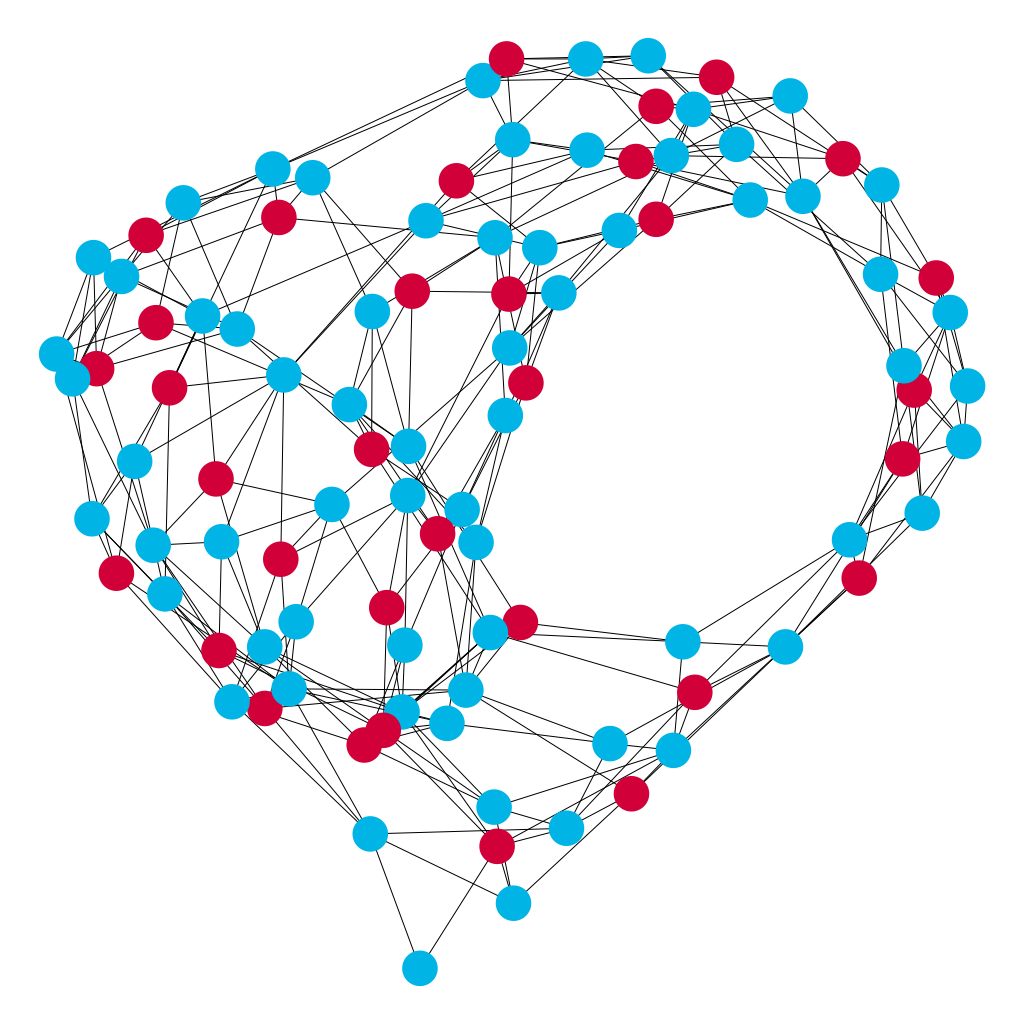
\includegraphics[scale=0.22]{imgs/Sim2E.png}
\caption{An interaction infrastructure where $\Delta(\Lambda)=0$ and $m=1.5$}
\label{Sim2}
\end{figure}

\subsubsection{Egalitarian exchange economy: Costly economic interaction}

The second set of simulations assume that there exists some costly inefficiencies for each economic interaction. Again, two simulations are conducted that correspond to the costless simulations above whereby the extent of the learning effects are altered. The first simulation assumes $m = 1$ and the second assumes $m = 1.5$. In both simulations we set the cost of forming an economic relationship at $\Delta(\Lambda) = 0.25$.

\paragraph{Simulation 1C : Costly interactions with equal learning effects.}

In the first simulation we find the existence of multiple equilibrium interaction infrastructures. One equilibrium is that of a monadic economy represented by an empty network, in which consumer-producers are indifferent to autarkically specialising in either $X$ or $Y$. In this case each consumer-producer earns a utility of $2$ in autarky. The other potential equilibrium is exactly the same as the first simulation in which pairs of economic interactions exist such that one consumer-producer specialises in the production of $X$ and the other specialises in the production of $Y$. Both equilibria are shown in Figure~\ref{Sim3}.

\begin{figure}[t]
\centering

\includegraphics[scale=0.22]{imgs/Sim3E.png}
\caption{An interaction infrastructure where $\Delta(\Lambda)=2$ and $m=1$}
\label{Sim3}
\end{figure}

\subsubsection{Cournot-Nash exchange economy: Costless economic interaction}

In these simulations we set $\Delta(\Lambda) = 0$. Prior to running the simulations we can note that, given the existence of an efficient trade mechanism where demand and supply are equalised, the use of a Cournot-Nash exchange mechanism leads to the following properties shown in Proposition~\ref{efficientSpec} below.

\begin{proposition} \label{efficientSpec}
Let there exist a Cournot-Nash exchange economy $\mathbb{E}_{C}$ such that $i,j \in N$. Assuming that $\Delta(\Lambda) = 0$ the following properties hold:
\begin{itemize}
	\item[(i)] All possible $ij$-interactions are mutually beneficial;
	\item[(ii)] The network that emerges is a complete network; and
	\item[(iii)] All consumer-producers are fully specialised in the production of a single output.
\end{itemize}
\end{proposition}

Proposition~\ref{efficientSpec} (ii) follows intuitively from (i), and Proposition~\ref{efficientSpec} (iii) is equivalent to Theorem~\ref{th:Spec}. The interaction network that emerges is analogous to a \emph{market} whereby all agents operate and trade with one another. Moreover, as interaction inefficiencies increase, the complete structure of the network can lose its integrity. This will be seen when considering the costly network formation below.

In the first simulation we set $m = 1$. As hypothesised in Proposition~\ref{efficientSpec} we find that a complete network emerges whereby agents that enter the socio-economic space specialise in a sequential manner such that agent 1 specialises in the production of $X$, agent 2 specialises in the production of $Y$, agent 3 specialises in the production of $X$, agent 4 specialises in the production of $Y$, and so on. The outcome of the simulation can be seen in Figure~\ref{Sim5}. We further note that the utilities of all agents converge.

\begin{figure}[t]
\centering

\includegraphics[scale=0.22]{imgs/Sim1C.png}
\caption{An interaction infrastructure where $\Delta(\Lambda)=0$ and $m=1$}
\label{Sim5}
\end{figure}

In the second simulation we set $m = 1.5$. Given that $\Delta(\Lambda) = 0$ the interaction inefficiency is minimal and thus a complete network is generated from the simulation of the Cournot-Nash exchange mechanism. Therefore, regardless of the production technology the topology of the interaction infrastructure remains unchanged. The only notable change is the proportion of agents specialising in the production of good $Y$, which increases due to the improved production abilities. Due to the lack of change with regards the structure we do not provide a corresponding Figure.

\subsubsection{Cournot-Nash exchange economy: Costly economic interaction}

The third simulation assesses costly network formation, in the form of positive interaction inefficiency, with equal production technologies for both goods $X$ and $Y$. We note that interaction inefficiencies are experienced on both sides of the economic interaction, not just the agent entering the socio-economic space and initiating the interaction. As a consequence, the network formation process follows a two-sided network formation model.

The result is the formation of a scale-free network with a degree distribution that follows a power law whereby the earliest entrants into the socio-economic space have the largest number of economic interactions. Due to the cost in forming economic interactions the and the production abilities of the individual agent the number of economic interactions per agent is limited unlike what was seen in the initial costless simulation, whereby the efficient price mechanism provided local price levels that benefited both parties when engaging in the economic trade. This limitation means that early entrants into the socio-economic space will engage in many exchanges as new agents enter the space; however, the number of their interactions will stop at some level. This will happen consecutively for all early economic agents thus leading to a structure with multiple hubs. These `hubbed' nodes are the earliest agents to enter the socio-economic space\footnote{We further note that a scale-free network is the natural market structure to emerge from adaptive specialisation. When simulating the emergence of an interaction infrastructure whereby agents could make only a limited number of economic interactions when entering the socio-economic space a scale-free network also emerged. A set limit on the number of economic interactions that can be formed forces individual economic agents to only form interactions with others that already have a large number of economic relations.}. Many empirical economic exchange networks also follow this scale-free structure \citep{Schweitzer2009}.

\begin{figure}[t]
\centering
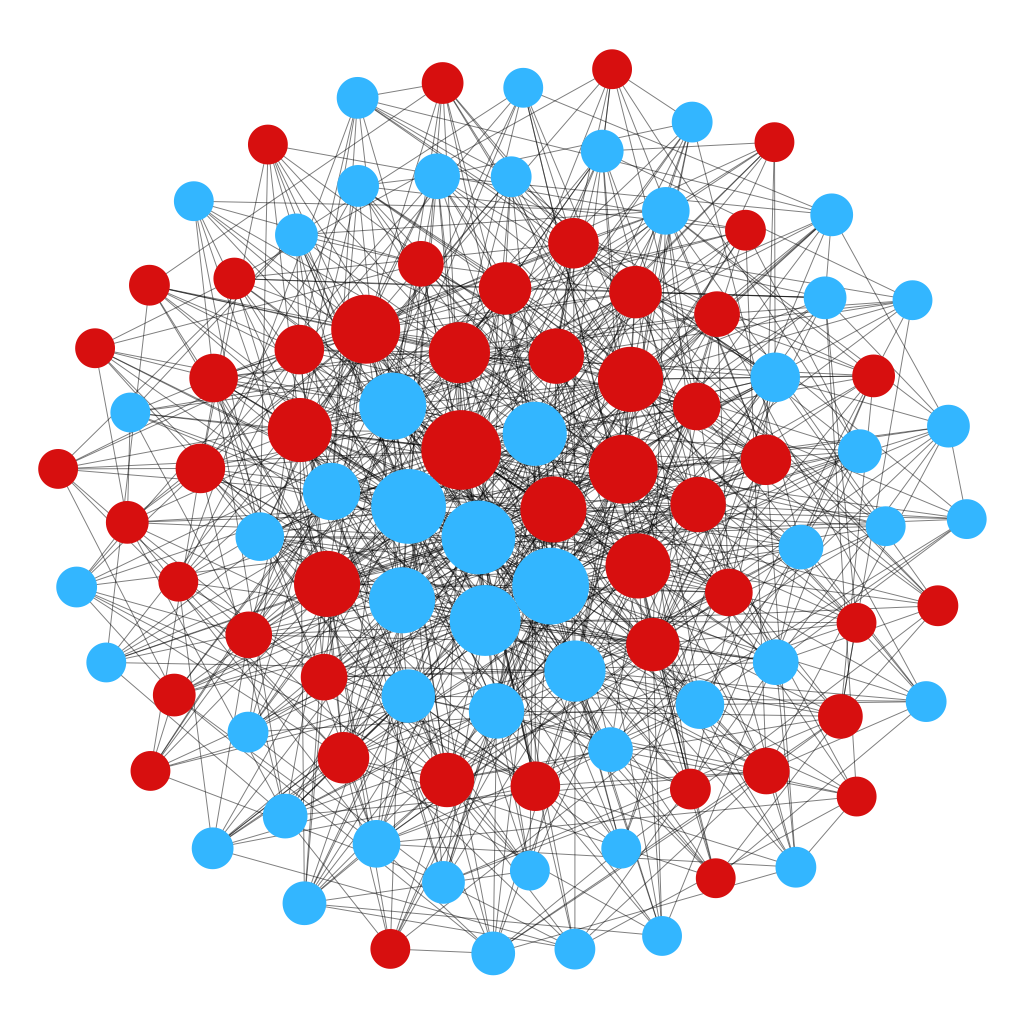
\includegraphics[scale=0.22]{imgs/Sim3C.png}
\caption{An interaction infrastructure where $\Delta(\Lambda)=0.2$ and $m=1$}
\label{Sim7}
\end{figure}

\subsubsection{Analysis of results} % (fold)
\label{sub:analysis_of_results}

% subsection analysis_of_results (end)

The representation between the interaction of elements of the socio-economic space shown in Figure~\ref{spacestructure} suggests that the institutions of a socio-economic space have a direct impact on the interaction infrastructures, which are formed by the economic interactions of a population of agents. The infrastructure is therefore a reflection of the state of the institutions and that entrepreneurship acts to alter the institutional environment, which is reflected in the interaction infrastructure itself. Our simulations of the socio-economic space based on the division of labour confirms the representation shown in Figure~\ref{spacestructure}. Specifically we model institutional and technological change in a number of ways. First, we note institutional change through changes in the interaction inefficiency, or transaction costs, of exchange between pairs of economic agents. In short we find that as the interaction inefficiency rises from $\Delta(\Lambda) = 0$ to some positive real number the number of \emph{structural holes} in the network increases and there emerges an increased distribution of utility throughout the network. These structural holes appear due to the reduced benefits of forming economic relationships with the entire population of agents. A natural consequence of the algorithm that solves the adaptive specialisation problem is that for all economic agents the next economic relationship formed will provide less benefit than the previous relationship: there is diminishing marginal benefit for each economic interaction. 

Whilst increasing the interaction inefficiency there will exist a tipping point whereby below this level of interaction inefficiency there will exist some wealth-generating relationships and above this tipping point there exists no economic relationships between agents. With regards the first egalitarian exchange economy: if $\Delta(\Lambda) > 0.25$ then an empty network will emerge; if $\Delta(\Lambda) < 0.25$ a minimally connected bipartite networks emerges; and if $\Delta(\Lambda) = 0.25$ then multiple equilibria can emerge as each agent is indifferent to forming an economic interaction with another agent. This notion of tipping points when regarding changes in interaction inefficiency has important implications for how we perceive the development of the socio-economic space. Indeed, substantial development may occur through punctuated events of tipping points. The structure of an institution may change thus facilitating a non-linear increase in the number of functional economic interactions and utility generated throughout the network.

When the interaction inefficiency tends to zero then there will exist a more homogenous socio-economic space such that each economic agent will derive a relatively equal utility and have a position in the networked structure that is structurally equivalent to all other agents in the space. For example, when the $\Delta(\Lambda) = 0$ for both the egalitarian exchange economy and the Cournot-Nash exchange economy each agent has the same level of utility and possess positions in the space that are structurally equivalent to all other agents. Thus, some agents may benefit more than others by maintaining the interaction inefficiency at a relatively high level.

Second, we note institutional change through changes in the exchange mechanism itself. Specifically we consider two exchange economies---the egalitarian exchange economy and the Cournot-Nash exchange economy---which obviously depends on the exchange mechanism used for trade. This is a more substantial change than simply a change in the interaction inefficiency experienced by agents to use the elements of the governance system to form economic interactions with each other. Moreover, a change in the exchange mechanism used may not lead to a change in the interaction inefficiency itself. Again, the exchange mechanism used has a substantial impact on the topology of the interaction infrastructure of the socio-economic space and the overall utilities of individual economic agents. The simulations showed that the use of a Cournot-Nash exchange mechanism was superior to the use of the egalitarian exchange mechanism in terms of the utility it generated for each individual agent.

Finally, we investigate change in the efficiency of production technologies through the variable $m$, which is connected to the efficiency regarding the production of good $Y$. An improvement in the production technologies of a given output may emerge from a reduction in role-building costs of the specific role that pertains to the output $Y$, or it may derive from an improvement of actual technological production. We find that as the efficiency of the production technology increases and agents become more productive in the production of good $Y$, more agents tend to specialise in the production of $Y$. Influencing a change to the production technology of some output leads to a change in the topology of the interaction infrastructure and the proportion of the population specialising in the production of the given output. Specifically, as $m$ increases, there will be more incentive for agents to specialise in the production of $Y$.

\paragraph{The impact of entrepreneurship.} % (fold)
\label{par:the_impact_of_entrepreneurship_}

% paragraph the_impact_of_entrepreneurship_ (end)

As noted in Definition~\ref{def:entrepreneur} above, entrepreneurship refers to the actions that modify in a major way elements of the governance system and the underlying interaction infrastructure of the socio-economic space. With respect to the simulations above, the transition from one exchange mechanism to another and technological advancements---the ability for individual economic agents to improve their production possibilities---relates to the process of entrepreneurship. 

We see that all institutional and technological changes discussed lead to major changes in the interaction infrastructure and society's utility. Both institutional changes---the reduction of interaction inefficiency for all agents and the change in the exchange mechanism used---are signs of entrepreneurial action. An improvement in production technologies can be more ambiguous if the change in production technologies is attributed to institutional changes itself. For example, if the improvement in production technologies is a consequence of a reduction in role-building costs for all agents due to, for example, the establishment of or improvement in educational institutions then this may be considered an act of entrepreneurship. If however, the improvement in production technology is isolated to the individual herself and not others in the socio-economic space then this will be considered the act of the entrepreneurial function. This conclusion regarding the regarding the scale of entrepreneurial action follows the same lines as Schumpeter, who claimed that an entrepreneur had a \emph{disequilibriating} impact on technological innovation. 

This short discussion of the entrepreneur and the resulting simulations provide an overview on the role of the entrepreneur and the impact of entrepreneurship within the relational perspective. Due to the importance of entrepreneurship and the lack of discussion and clarity on the topic of the entrepreneur in traditional economic literature we provide a further discussion in Chapter~\ref{ch:entrepreneurship}. In the subsequent discussion we draw an important link between the act of entrepreneurship and the generation of new socio-economic roles and unique, and potentially exploitative, positions within the socio-economic space.
